%---------------------------------------------------------------------------------------------------------------------------- 
\graphicspath{{Parti/P03-Meccanica_SR/C01-Cinematica_CR/Figure/}}
\chapter{Cinematica infinitesima del corpo rigido}\label{cap:cinematica_infinitesima}
%---------------------------------------------------------------------------------------------------------------------------- 

\begin{sommario}
	\todo{Da rivedere}
	Si introducono i gradi di libertà del corpo rigido, nello
	spazio e nel piano, come proprietà del vincolo di rigidità
	indipendente dall'ipotesi di spostamenti infinitesimi. Si
	deriva poi la formula fondamentale della cinematica
	infinitesima con due approcci indipendenti: la
	linearizzazione della rotazione finita --- sviluppata
	dapprima nel caso piano e poi estesa allo spazio --- e il
	principio di invarianza delle distanze. Si presenta la forma
	matriciale, con la sua restrizione al caso piano. Si studiano
	gli invarianti del campo di spostamento e si introduce l'asse
	centrale degli spostamenti con una costruzione geometrica. Si
	classificano i moti rigidi infinitesimi e si specializza la
	trattazione al caso piano, con la determinazione del centro
	di rotazione. Si conclude con la relazione fra spostamenti
	infinitesimi e campo di velocità.
\end{sommario}



\section{Il corpo rigido e il campo di spostamento}\label{sez.CR}
Non daremo nella nostra trattazione una definizione di corpo, ma piuttosto lo assumeremo come un ente primitivo.
Assumiamo  che i corpi possano avere diverse configurazioni, occupando diverse regioni dello spazio Euclideo $\Ec$; identifichiamo dunque un corpo con una delle sue possibili configurazioni $\Cc$, ovvero una regione limitata e regolare di $\Ec$, i cui elementi sono punti.

Il corpo $\Cc$ può subire una certa trasformazione, andando ad occupare una differente regione $\Cc_*$ dello spazio; indichiamo con $P_*$ l'immagine del punto $P$ sotto la trasformazione che manda $\Cc$ in $\Cc_*$ (v. Fig. \ref{fig:displ}). Fissata una volta per tutte un'origine $O$ dello spazio Euclideo, se il punto $P$ aveva inizialmente posizione $\overrightarrow{OP}=:\xb(P)$, dopo la trasformazione avrà posizione $\overrightarrow{OP_*}=:\xb(P_*)$. 

\begin{figure}
	\centering
	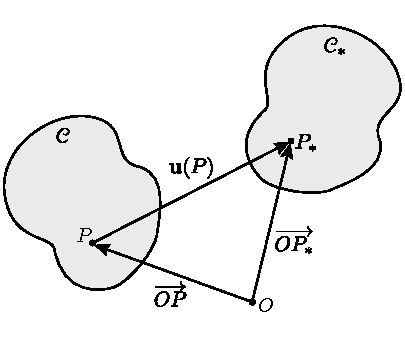
\includegraphics[scale=1]{Parti/P03-Meccanica_SR/C01-Cinematica_CR/Figure/displ}
	\caption{Due differenti configurazioni del corpo $\Cc$. }
	\label{fig:displ}
\end{figure}

Lo \textit{spostamento} del punto $P$ è definito come
\begin{equation}\label{displ}
	\ub(P):=P_*-P=\overrightarrow{OP_*}-\overrightarrow{OP},
\end{equation}
ovvero il vettore che porta $P$ in $P_*$. 

Un corpo è \textit{rigido} se, presi due qualunque punti $P, Q \in\Cc$, la loro mutua distanza resta invariata dopo una qualunque cambiamento di configurazione:
\begin{equation}\label{CR}
	|\overrightarrow{PQ}|=|\overrightarrow{P_*Q_*}| \qquad \forall P,Q\in\Cc.
\end{equation}

Questa condizione, in virtù della \eqref{displ}, pone delle restrizioni sulla possibile forma che il campo di spostamento può avere. In particolare, la  \eqref{CR} 
è equivalente a 
\begin{equation}\label{eq:rigidita_esatta}
	\bigl|\overrightarrow{PQ}\bigr|^2=|Q_*-P_*|^2=|Q+\ub(Q)-P-\ub(P)|^2=\bigl|\overrightarrow{PQ} + \ub(Q) - \ub(P)\bigr|^2,
\end{equation}
ovvero, sviluppando il quadrato del secondo membro:
\begin{equation}\label{eq:rigidita_sviluppo}
	\bigl|\overrightarrow{PQ}\bigr|^2=\bigl|\overrightarrow{PQ}\bigr|^2 
	+ 2\,\overrightarrow{PQ} \cdot \bigl[\ub(Q) - \ub(P)\bigr]
	+ \bigl|\ub(Q) - \ub(P)\bigr|^2
\end{equation}
da cui:
%Semplificando $|\overrightarrow{PQ}|^2$:
\begin{equation}\label{eq:rigidita_semplificata}
	2\,\overrightarrow{PQ} \cdot \bigl[\ub(Q) - \ub(P)\bigr]
	+ \bigl|\ub(Q) - \ub(P)\bigr|^2 = 0.
\end{equation}

Dividendo per $|\overrightarrow{PQ}|^2$, otteniamo la condizione
\begin{equation}\label{eq:rigidita_adim}
	2\,\ab_{PQ} \cdot \bm{\updelta}_{PQ} + |\bm{\updelta}_{PQ}|^2 = 0,
\end{equation}
dove $\ab_{PQ} = \overrightarrow{PQ}/|\overrightarrow{PQ}|$ è il versore di $\overrightarrow{PQ}$ e
\begin{equation}
	\bm{\updelta}_{PQ} \coloneqq \frac{\ub(Q)-\ub(P)}{|\overrightarrow{PQ}|}.
\end{equation}

Osserviamo che $|\bm{\updelta}_{PQ} |$ confronta l'ampiezza dello spostamento relativo di due punti con la loro distanza iniziale, facilmente interpretabile, alla luce di \eqref{displ}, come 
\begin{equation}
	|\bm{\updelta}_{PQ} |=\frac{\left|\overrightarrow{P_*Q_*}-\overrightarrow{PQ}\right|}{|\overrightarrow{PQ}|},
\end{equation}
ovvero come una  misura della variazione relativa della configurazione.

Ha senso dunque sviluppare una \textit{teoria infinitesima}, che richieda che questa quantità sia `piccola', ovvero che la configurazione cambi di poco rispetto a quella di riferimento. 
Dato che $|\bm{\updelta}_{PQ} |$ dipende dai punti $P, Q$, individuiamo la massima variazione relativa di configurazione, ovvero
\begin{equation}\label{sup}
	\delta:=\sup_{P, Q	\in\Cc} |\bm{\updelta}_{PQ} |
\end{equation}
e consideriamo un'espansione  in serie di Taylor al primo ordine, trascurando dunque  tutti i termini di ordine $\delta^2$. Vista la \eqref{sup}, senz'altro
\begin{equation}
	\left|\bm{\updelta}_{PQ}\right|\leq \delta \quad \forall P,Q\in \Cc
\end{equation}
e dunque siamo autorizzati a trascurare nella \eqref{eq:rigidita_adim} il termine dell'ordine di $|\bm{\updelta}_{PQ}|^2$.

Concludiamo che, in teoria infinitesima, la conseguenza della condizione di rigidità è 
%
%\vspace{2cm}
%Per valutare il peso relativo dei due termini, dividiamo per 
%$|\overrightarrow{PQ}|^2$, introducendo il versore 
%$\ab_{PQ} = \overrightarrow{PQ}/|\overrightarrow{PQ}|$ e lo 
%\textit{spostamento relativo adimensionalizzato} 
%$\bm{\updelta}_{PQ} = [\ub(Q)-\ub(P)]/|\overrightarrow{PQ}|$:
%\begin{equation}\label{eq:rigidita_adim}
%2\,\ab_{PQ} \cdot \bm{\updelta}_{PQ} + |\bm{\updelta}_{PQ}|^2 = 0.
%\end{equation}
%
%\vspace{1cm}
%\todo[inline]{Riscivere la parte sotto}
%Il parametro $|\bm{\updelta}_{PQ}|$ confronta lo spostamento relativo con la 
%distanza fra i due punti: è il rapporto fra la variazione di posizione 
%relativa e la dimensione caratteristica del corpo. La condizione di 
%\textit{spostamenti infinitesimi}\index{spostamento!infinitesimo|textbf} consiste nel richiedere che
%\begin{equation}
%|\bm{\updelta}_{PQ}| = \frac{|\ub(Q)-\ub(P)|}{|\overrightarrow{PQ}|} \ll 1
%\qquad \forall\, P,\, Q,
%\end{equation}
%ovvero che gli spostamenti relativi siano piccoli rispetto alle distanze 
%fra i punti del corpo. Sotto questa ipotesi il termine $|\bm{\updelta}_{PQ}|^2$ 
%nella~\eqref{eq:rigidita_adim} è trascurabile rispetto al termine 
%$2\,\ab_{PQ} \cdot \bm{\updelta}_{PQ}$, che è del primo ordine in 
%$|\bm{\updelta}_{PQ}|$. La condizione di rigidità linearizzata è dunque
\begin{equation}\label{eq:ortogonalita_CR}
	\overrightarrow{PQ} \cdot \bigl[\ub(Q) - \ub(P)\bigr] = 0
	\qquad \forall\, P,\, Q.
\end{equation}

%%%%%%%%%%%%%%%%%%%%%%%%%%%%%%%%%%%%%%%%%%%%%%%%%%%%%%%%%%%
\begin{figure}[!htbp]
	\centering
	\usetikzlibrary{arrows.meta,calc,decorations.markings}
	
	% --- helper per le figure ---
	\tikzset{midarrow/.style={postaction={decorate},
			decoration={markings, mark=at position 0.56 with {\arrow{Stealth}}}}}
	
	\newcommand{\rightangle}[3]{%
		\coordinate (ra1) at ($(#2)!2mm!(#1)$);
		\coordinate (ra3) at ($(#2)!2mm!(#3)$);
		\draw[line width=0.4pt] (ra1) -- ($(ra1)+(ra3)-(#2)$) -- (ra3);}
	\resizebox{0.9\textwidth}{!}{%
		\begin{tikzpicture}[>=Stealth, line width=0.8pt, scale=0.95,
			pt/.style={circle,fill,inner sep=1.3pt},
			open/.style={circle,draw,line width=0.6pt,inner sep=1.1pt}]
			\coordinate (O)  at (1.8,-0.5);
			\coordinate (P)  at (0,0.5);
			\coordinate (Q)  at (3.4,1.2);
			\coordinate (aA) at (3.645,1.250);
			\coordinate (aB) at (4.477,1.422);
			\coordinate (Ps) at (0.770,1.221);
			\coordinate (Qs) at (3.938,3.047);
			\coordinate (QuP) at (4.170,1.921);
			
			\draw[->, thin] (O) -- (P) node[pos=0.5,below left=-3pt] {$\xb_P$};
			\draw[->, thin] (O) -- (Q) node[pos=0.5,below right=-3pt] {$\xb_Q$};
			
			\draw[thick, midarrow] (P) -- (Q) node[pos=0.6,below=2pt] {$\overrightarrow{PQ}$};
			%\draw[->, thick] (aA) -- (aB) node[pos=0.97,above=1pt] {$\ab_{PQ}$};
			
			% retta d'azione di PQ (grigia) da Q verso destra
			\draw[gray!60] (Q) -- ($(P)!1.62!(Q)$);
			
			% versore a_PQ (nero) disegnato su quella retta
			\coordinate (aA) at ($(P)!1.28!(Q)$);
			\coordinate (aB) at ($(P)!1.52!(Q)$);
			\draw[->, thick] (aA) -- (aB) node[pos=0.97,below=1pt] {$\ab_{PQ}$};
			
			\draw[thin, midarrow] (Ps) -- (QuP);   % chiude il parallelogramma P Q (Q+u_P) P*
			
			\draw[->, thick] (P) -- (Ps) node[pos=0.5,above left=-3pt] {$\ub_P$};
			\draw[thick, midarrow] (Q) -- (Qs) node[pos=0.5,left=1pt] {$\ub_Q$};
			\draw[thick, midarrow] (Q) -- (QuP) node[pos=0.55,below right=-6pt] {$\ub_P$};
			\draw[thick, midarrow] (QuP) -- (Qs) node[pos=0.5,right=1pt] {$\ub_Q-\ub_P$};
			
			\draw[thick, midarrow] (Ps) -- (Qs) node[pos=0.5,above left=-2pt] {$\overrightarrow{P_*Q_*}$};
			
			\node[open,label={below:$O$}] at (O) {};
			\node[pt,label={left:$P$}]  at (P) {};
			\node[pt,label={[xshift=2pt]below right:$Q$}] at (Q) {};
			\node[pt,label={[yshift=1pt]above :$P_*$}]  at (Ps) {};
			\node[pt,label={ above:$Q_*$}] at (Qs) {};
			
			\node at (3.6,-1.0) {(a)};
		\end{tikzpicture}
		\quad
		% ---- pannello (b) ----
		\begin{tikzpicture}[>=Stealth, line width=0.8pt, scale=0.95,
			pt/.style={circle,fill,inner sep=1.3pt},
			open/.style={circle,draw,line width=0.6pt,inner sep=1.1pt}]
			\coordinate (O)  at (1.8,-0.5);
			\coordinate (P)  at (0,0.5);
			\coordinate (Q)  at (3.4,1.2);
			\coordinate (aA) at (3.645,1.250);
			\coordinate (aB) at (4.477,1.422);
			\coordinate (Ps) at (0.770,1.221);
			\coordinate (Qs) at (3.938,3.047);
			\coordinate (QuP) at (4.170,1.921);
			\coordinate (FP) at (0.881,0.682);
			\coordinate (FQ) at (4.281,1.382);
			
			\draw[->, thin] (O) -- (P) node[pos=0.5,below left=-3pt] {$\xb_P$};
			\draw[->, thin] (O) -- (Q) node[pos=0.5,below right=-3pt] {$\xb_Q$};
			
			\draw[thick, midarrow] (P) -- (Q) node[pos=0.42,above=1pt] {$\overrightarrow{PQ}$};
			%\draw[->, thick] (aA) -- (aB) node[pos=0.97,above=1pt] {$\ab_{PQ}$};
			% retta d'azione di PQ (grigia) da Q verso destra
			\draw[gray!60] (Q) -- ($(P)!1.62!(Q)$);
			
			% versore a_PQ (nero) disegnato su quella retta
			\coordinate (aA) at ($(P)!1.28!(Q)$);
			\coordinate (aB) at ($(P)!1.52!(Q)$);
			\draw[->, thick] (aA) -- (aB) node[pos=0.97,above=1pt] {$\ab_{PQ}$};
			
			% proiezioni grigie tratteggiate (PRIMA di u_Q-u_P) + angoli retti
			\draw[dashed, gray!60] (Ps) -- (FP);
			\draw[dashed, gray!60] (Qs) -- (FQ);
			\rightangle{P}{FP}{Ps}
			\rightangle{aB}{FQ}{Qs}
			
			% spostamenti (DOPO: sovrascrivono il grigio)
			\draw[->, thick] (P) -- (Ps) node[pos=0.5,above left=-3pt] {$\ub_P$};
			\draw[thick, midarrow] (Q) -- (Qs) node[pos=0.5,left=1pt] {$\ub_Q$};
			\draw[->, thick] (Q) -- (QuP);
			\draw[thick, midarrow] (QuP) -- (Qs) node[pos=0.5,right=1pt] {$\ub_Q-\ub_P$};
			
			% etichette delle proiezioni collegate con una freccia di richiamo
			%\node (lpP) at (1.85,0.02) {$\ub_P\!\cdot\ab_{PQ}$};
			%\draw[gray!60] (P) -- (FP);
			\node (lpP) at (1.80,0.45) {$\ub_P\!\cdot\ab_{PQ}$};
			\draw[->, thin] (lpP) -- ($(P)!0.45!(FP)$);
			\node (lpQ) at (4.75,0.72) {$\ub_Q\!\cdot\ab_{PQ}$};
			\draw[->, thin] (lpQ) -- ($(Q)!0.5!(FQ)$);
			
			\node[open,label={below:$O$}] at (O) {};
			\node[pt,label={left:$P$}]  at (P) {};
			\node[pt,label={[xshift=2pt]above left:$Q$}] at (Q) {};
			\node at (3.6,-1.0) {(b)};
		\end{tikzpicture}
	}
	\caption{(a)~Spostamenti rigidi e (b)~interpretazione geometrica della condizione di ortogonalità fra il vettore posizione relativo $\protect\overrightarrow{PQ}$ e il vettore relativo degli spostamenti infinitesimi $\ub_Q - \ub_P$.}
	\label{fig:orto_PQ_spost_relat}
\end{figure}
%%%%%%%%%%%%%%%%%%%%%%%%%%%%%%%%%%%%%%%%%%%%%%%%%%%%%%%%%%%
Questa condizione di \textit{ortogonalità} fra il vettore congiungente e 
lo spostamento relativo ha un significato geometrico limpido: le proiezioni 
di $\ub(P)$ e $\ub(Q)$ lungo la direzione che congiunge i due punti sono 
uguali. In altre parole, i due punti si spostano della stessa quantità nella 
direzione $\overrightarrow{PQ}$; ciò che può differire è solo la componente 
dello spostamento perpendicolare alla congiungente, che non altera la distanza 
(al primo ordine, cfr.~\FIGref{fig:orto_PQ_spost_relat}(b)).
Questa proprietà prende il nome di \textit{equiproiettività}\index{equiproiettivita@equiproiettività|textbf}
del campo degli spostamenti rigidi: in formule,
$\ub(P) \cdot \ab_{PQ} = \ub(Q) \cdot \ab_{PQ}$ per ogni
coppia di punti, dove
$\ab_{PQ} = \overrightarrow{PQ}/|\overrightarrow{PQ}|$. 






\subsection{Rappresentazione del campo di spostamento}\label{sez:rappresentazione_campo}

Dalla condizione \eqref{eq:ortogonalita_CR} segue un importante risultato, che caratterizza in maniera specifica il campo di spostamento di un corpo rigido in teoria infinitesima.
Fissiamo un punto $P$ e indichiamo con $\wb_P(Q)\coloneqq \ub(Q)-\ub(P)$ lo  spostamento relativo  rispetto a $P$, per qualunque $Q\in\Cc$. La condizione \eqref{eq:ortogonalita_CR}  è $\overrightarrow{PQ}\cdot \wb_P(Q)=0$, per ogni $Q\in \Cc$. Prendiamo adesso due punti arbitrari $Q,R$, per cui vale
\begin{equation}
	\begin{aligned}
		0=&\overrightarrow{QR}\cdot[\ub(R)-\ub(Q)]=(\overrightarrow{PR}-\overrightarrow{PQ})\cdot [\big(\ub(R)-\ub(P)\big)-\big( \ub(Q)-\ub(P) \big)]\\
		=&\overrightarrow{PR}\cdot \wb_P(R)-\overrightarrow{PR}\cdot \wb_P(Q)-\overrightarrow{PQ}\cdot\wb_P(R)+\overrightarrow{PQ}\cdot \wb_P(Q).
	\end{aligned}
\end{equation}
Il primo e l'ultimo termine della seconda riga sono nulli, per la condizione di equiproiettività. Ne segue che
\begin{equation}\label{eq:bilineare_wP}
	\overrightarrow{PR}\cdot \wb_P(Q)+\overrightarrow{PQ}\cdot\wb_P(R)=0 \qquad \forall\, Q,R\in\Cc.
\end{equation}

\paragraph{Linearità di $\wb_P$.}
Scegliamo $P$ interno a $\Cc$ (è sempre possibile, essendo $\Cc$ una regione regolare) e una base ortonormale $\ab_x,\ab_y,\ab_z$. Poiché $P$ è interno, esiste $\varepsilon>0$ tale che i tre punti $R_i\in\Cc$ tali che $\overrightarrow{PR_i}=\varepsilon\,\ab_i$ ($i=x,y,z$) sono ben definiti. Ponendo $R=R_i$ nella \eqref{eq:bilineare_wP}:
\begin{equation}
	\varepsilon\,\ab_i\cdot \wb_P(Q) + \overrightarrow{PQ}\cdot \wb_P(R_i) = 0
	\;\Longrightarrow\;
	\ab_i\cdot \wb_P(Q) = -\overrightarrow{PQ}\cdot \wb_i, \qquad i=x,y,z,
\end{equation}
dove $\wb_i:=\wb_P(R_i)/\varepsilon$ sono vettori \emph{fissati}, indipendenti da $Q$ (ma costruiti a partire dal polo $P$). 
Abbiamo così determinato, per ogni $Q\in\Cc$, le tre componenti del vettore $\wb_P(Q)$ lungo la base ortonormale $\ab_x,\ab_y,\ab_z$. Ricordando che un vettore $\vb$ qualunque si ricostruisce dalle sue componenti su una base ortonormale tramite l'identità $\vb=\sum_i(\ab_i\cdot\vb)\,\ab_i$, applichiamo questo fatto a $\vb=\wb_P(Q)$ e sostituiamo le tre componenti appena trovate:
\begin{equation}\label{eq:linearita_wP}
	\wb_P(Q) = \sum_{i=x,y,z}\bigl(\ab_i\cdot\wb_P(Q)\bigr)\,\ab_i
	= -\sum_{i=x,y,z}\bigl(\overrightarrow{PQ}\cdot\wb_i\bigr)\,\ab_i
	=: \bm{\Theta}_P\,\overrightarrow{PQ}, \qquad \forall\, Q\in\Cc,
\end{equation}
dove $\bm{\Theta}_P$ è il tensore di componenti $(\Theta_P)_{ij}=-(\wb_i)_j$ (la componente $j$-esima del vettore $\wb_i$).
La \eqref{eq:linearita_wP} mostra che $\wb_P(Q)$ dipende \emph{linearmente} da $\overrightarrow{PQ}$, tramite un tensore $\bm{\Theta}_P$ che non dipende da $Q$ (per il fissato polo $P$). 


\paragraph{Antisimmetria di $\bm{\Theta}_P$.}
Sostituendo la \eqref{eq:linearita_wP} nella condizione di equiproiettività $\overrightarrow{PQ}\cdot\wb_P(Q)=0$, valida per ogni $Q\in\Cc$, si ottiene
\begin{equation}\label{eq:quadratica_nulla}
	\overrightarrow{PQ}\cdot \bm{\Theta}_P\,\overrightarrow{PQ} = 0 \qquad \forall\, Q\in\Cc.
\end{equation}
Applicando la \eqref{eq:quadratica_nulla} al punto $Q=R_i$ (per cui $\overrightarrow{PQ}=\varepsilon\ab_i$) e dividendo per $\varepsilon^2$:
\begin{equation}
	(\Theta_P)_{ii} = 0, \qquad i=x,y,z:
\end{equation}
le componenti diagonali di $\bm{\Theta}_P$ sono nulle. Essendo $P$ interno a $\Cc$, possiamo scegliere (eventualmente riducendo $\varepsilon$) anche tre punti $R_{ij}\in\Cc$, con $i\neq j$, tali che $\overrightarrow{PR_{ij}}=\varepsilon(\ab_i+\ab_j)$. Applicando la \eqref{eq:quadratica_nulla} a $Q=R_{ij}$ e dividendo per $\varepsilon^2$:
\begin{equation}
	0=(\ab_i+\ab_j)\cdot \bm{\Theta}_P(\ab_i+\ab_j)
	= \underbrace{\ab_i\cdot \bm{\Theta}_P\ab_i}_{=0} + \ab_i\cdot \bm{\Theta}_P\ab_j+\ab_j\cdot \bm{\Theta}_P\ab_i+\underbrace{\ab_j\cdot \bm{\Theta}_P\ab_j}_{=0},
\end{equation}
cioè $(\Theta_P)_{ij}+(\Theta_P)_{ji}=0$ per ogni $i\neq j$. Insieme all'annullarsi della diagonale, questo significa esattamente che $\bm{\Theta}_P$ è antisimmetrico: $(\Theta_P)_{ji}=-(\Theta_P)_{ij}$ per ogni $i,j=x,y,z$.


Ogni tensore antisimmetrico $\bm{\Theta}_P$, in dimensione 3, si scrive in modo unico come $\bm{\Theta}_P\mb=\bm{\upvartheta}_P\times\mb$ per ogni $\mb$, per un opportuno vettore $\bm{\upvartheta}_P$\footnote{Di componenti $(\vartheta_P)_k=-\tfrac12\varepsilon_{kij}(\Theta_P)_{ij}$, dove $\varepsilon$ è il simbolo di Ricci (v.  Sez. \ref{prodvet}).}. Dalla \eqref{eq:linearita_wP} segue allora
\begin{equation}\label{eq:formula_polo_P}
	\ub(Q)-\ub(P) = \wb_P(Q) = \bm{\upvartheta}_P\times\overrightarrow{PQ} \qquad \forall\, Q\in\Cc.
\end{equation}

\paragraph{Indipendenza di $\bm\upvartheta_P$ dal polo.}
Il vettore $\bm\upvartheta_P$ trovato dipende, a priori, dal polo $P$. Sia $P'\in\Cc$ un altro polo, con vettore associato $\bm\upvartheta_{P'}$. Per ogni $Q\in\Cc$, usando $\overrightarrow{P'Q}-\overrightarrow{P'P}=\overrightarrow{PQ}$,
\begin{equation}
	\begin{aligned}
		\bm\upvartheta_P\times\overrightarrow{PQ} &= \ub(Q)-\ub(P)
		= \bigl[\ub(Q)-\ub(P')\bigr]-\bigl[\ub(P)-\ub(P')\bigr]\\
		&= \bm\upvartheta_{P'}\times\overrightarrow{P'Q}-\bm\upvartheta_{P'}\times\overrightarrow{P'P}
		= \bm\upvartheta_{P'}\times\overrightarrow{PQ}.
	\end{aligned}
\end{equation}
Dunque $(\bm\upvartheta_P-\bm\upvartheta_{P'})\times\overrightarrow{PQ}=\mathbf 0$ per ogni $Q\in\Cc$; poiché, al variare di $Q$ in un intorno di $P$, $\overrightarrow{PQ}$ assume almeno due direzioni non parallele, l'unica possibilità è $\bm\upvartheta_P=\bm\upvartheta_{P'}$. Il vettore $\bm\upvartheta$ è dunque lo stesso per ogni scelta del polo. In particolare, se $P$ è un punto di bordo di $\Cc$ (per cui l'argomento precedente non si applica direttamente, mancando un intorno di $P$ interamente in $\Cc$), fissato un qualunque $P_0$ interno si ha comunque $\ub(Q)=\ub(P_0)+\bm\upvartheta\times\overrightarrow{P_0Q}$ per ogni $Q\in\Cc$, bordo compreso; applicando questa relazione sia a $Q$ sia a $P$ e sottraendo, come nel conto sopra, si ottiene $\ub(Q)-\ub(P)=\bm\upvartheta\times\overrightarrow{PQ}$ anche in questo caso.

Concludiamo dunque che 
\begin{equation}\label{eq:campo_rigido}
	\ub(Q) = \ub(P) + \bm{\upvartheta}\times \overrightarrow{PQ} \qquad \forall\, P,Q \in \Cc,
\end{equation}
ovvero, in termini del tensore antisimmetrico $\bm{\Theta}$ associato a $\bm\upvartheta$:
\begin{equation}\label{eq:campo_rigidoTH}
	\ub(Q) = \ub(P) + \bm{\Theta}\, \overrightarrow{PQ} \qquad \forall\, P,Q \in \Cc.
\end{equation}




% ============================================================
\subsection{La rotazione infinitesima}\label{sez:interpretazione}
% ============================================================

La formula \eqref{eq:campo_rigido} mostra che, fissato un polo $P$, l'intero spostamento relativo degli altri punti del corpo è determinato dal singolo vettore $\bm\upvartheta$ tramite il prodotto vettoriale $\bm\upvartheta\times\overrightarrow{PQ}$. Vogliamo ora mostrare che questa è esattamente la struttura di una rotazione infinitesima: la direzione di $\bm\upvartheta$ è l'asse, e il suo modulo è l'angolo (infinitesimo) di rotazione.

\medskip


Verifichiamo anzitutto che la \eqref{eq:campo_rigido} sia compatibile con la rigidità di partenza, cioè che spostare $Q$ rispetto a $P$ secondo questa formula non alteri (al primo ordine) la loro distanza. La nuova posizione relativa è
\begin{equation}
	\overrightarrow{P_*Q_*} = (Q+\ub(Q))-(P+\ub(P)) = \overrightarrow{PQ} + \bigl[\ub(Q)-\ub(P)\bigr] = \overrightarrow{PQ} + \bm\upvartheta\times\overrightarrow{PQ},
\end{equation}
usando la \eqref{eq:campo_rigido}. Poiché il prodotto misto $\overrightarrow{PQ}\cdot(\bm\upvartheta\times\overrightarrow{PQ})$ è nullo (è il prodotto misto di due vettori uguali), si ha esattamente
\begin{equation}
\begin{aligned}
		|\overrightarrow{P_*Q_*}|^2 &= \bigl|\overrightarrow{PQ}+\bm\upvartheta\times\overrightarrow{PQ}\bigr|^2
	= |\overrightarrow{PQ}|^2 + 2\,\overrightarrow{PQ}\cdot(\bm\upvartheta\times\overrightarrow{PQ}) + |\bm\upvartheta\times\overrightarrow{PQ}|^2\\
	&= |\overrightarrow{PQ}|^2 + |\bm\upvartheta\times\overrightarrow{PQ}|^2.
\end{aligned}
\end{equation}
 Resta da mostrare che il termine correttivo $|\bm\upvartheta\times\overrightarrow{PQ}|^2$ sia trascurabile. Ricordiamo che, per costruzione, i vettori $\wb_i=\wb_P(R_i)/\varepsilon$ da cui $\bm\upvartheta$ è stato ottenuto coincidono con $\bm\updelta_{PR_i}$  e dunque $|\wb_i|\leq\delta$ per definizione di $\delta$ come estremo superiore. Poiché le componenti di $\bm\Theta_P$ sono $(\Theta_P)_{ij}=-(\wb_i)_j$ e quelle di $\bm\upvartheta$ sono combinazioni lineari finite di queste, anche $|\bm\upvartheta|$ è controllato da $\delta$. Segue che
\begin{equation}
	|\bm\upvartheta\times\overrightarrow{PQ}|^2 \leq |\bm\upvartheta|^2|\overrightarrow{PQ}|^2 = O(\delta^2)\,|\overrightarrow{PQ}|^2,
\end{equation}
lo stesso ordine $\delta^2$ già trascurato in tutta la teoria infinitesima. La distanza $|\overrightarrow{PQ}|$ resta dunque invariata a meno di termini di questo ordine: siamo dunque di fronte ad una trasformazione che, al primo ordine, è un'isometria infinitesima. 




Questo però dice solo che non c'è deformazione, non ancora che si tratti di una rotazione attorno a un asse: potrebbe in linea di principio trattarsi di un'altra isometria. Per stabilirlo, calcoliamo esplicitamente l'azione di una rotazione finita — nota dalla geometria elementare — e poi la linearizziamo, per confrontarla direttamente con la \eqref{eq:campo_rigido}. 



\paragraph{Il caso piano.}
Consideriamo dapprima uno spostamento rigido piano: il campo di spostamento è parallelo a un piano fisso e indipendente dalla coordinata ortogonale ad esso. Scelto il piano $(x,y)$, il punto $O$, solidale al corpo, subisce una traslazione $\ub(O)$; il corpo ruota inoltre di un angolo $\vartheta$\nomenclature[G]{$\vartheta$}{angolo di una rotazione finita} attorno a $O$. La posizione di un generico punto $P$ dopo lo spostamento\nomenclature[L]{$\xb(P)$}{vettore posizione del punto $P$} è:
\begin{equation}\label{eq:pos_finale_piano}
	\xb(P) + \ub(P) = \xb(O) + \ub(O)
	+ \Rbb(\vartheta)\,\overrightarrow{OP},
\end{equation}
dove $\Rbb(\vartheta)$ è l'applicazione lineare di rotazione\nomenclature[L]{$\Rbb(\vartheta)$}{applicazione lineare di rotazione finita (di angolo $\vartheta$)} nel piano, la cui
matrice nella base $\{\ab_x,\ab_y\}$ è:
\begin{equation}\label{eq:R_piano}
	\bm{R}(\vartheta) = \begin{bmatrix}
		\cos\vartheta & -\sin\vartheta \\
		\sin\vartheta & \cos\vartheta
	\end{bmatrix}.
\end{equation}
Lo spostamento di $P$ è dunque
\begin{equation}\label{eq:spost_finito_piano}
	\ub(P) = \ub(O) + \bigl(\Rbb(\vartheta) - \Ib\bigr)\,\overrightarrow{OP}.
\end{equation}
Il termine $\bigl(\Rbb - \Ib\bigr)\,\overrightarrow{OP}$ è lo
spostamento di $P$ dovuto alla sola rotazione attorno a $O$. Per
comprenderne il significato geometrico, decomponiamo questo vettore
nella direzione di $\overrightarrow{OP}$ (componente radiale) e nella
direzione perpendicolare $\ab_z \times \overrightarrow{OP}$ (componente
tangenziale). Sviluppando il prodotto matriciale con
la~\eqref{eq:R_piano} si verifica che:
\begin{equation}\label{eq:R-I_piano}
	\bigl(\Rbb - \Ib\bigr)\,\overrightarrow{OP}
	= \sin\vartheta\;(\ab_z \times \overrightarrow{OP})
	+ (\cos\vartheta - 1)\;\overrightarrow{OP}.
\end{equation}
I due termini hanno un'interpretazione immediata (cfr.~\FIGref{fig:spostamenti_finiti}):
\begin{itemize}[nosep]
	\item $\sin\vartheta\;(\ab_z \times \overrightarrow{OP})$ è la
	componente \textit{tangenziale}: perpendicolare a $\overrightarrow{OP}$,
	nel verso della rotazione, di modulo $|\overrightarrow{OP}|\sin\vartheta$;
	\item $(\cos\vartheta - 1)\;\overrightarrow{OP}$ è la componente
	\textit{radiale}: diretta verso $O$ (poiché $\cos\vartheta - 1 \leq 0$),
	di modulo $|\overrightarrow{OP}|\,(1-\cos\vartheta)$.
\end{itemize}
%%%%%%%%%%%%%%%%%%%%%%%%%%%%%%%%%%%%%%%%%%%%%%%%%%%%%%%%%%%
\begin{figure}[!ht]
	\centering
	\tikzset{midarrow/.style={postaction={decorate},
			decoration={markings, mark=at position 0.55 with {\arrow{Stealth}}}}}
	\resizebox{0.90\textwidth}{!}{%
		\begin{tikzpicture}[>=Stealth, line width=0.8pt, scale=1.2,
			pt/.style={circle,fill,inner sep=1.3pt}]
			
			%==================== PANNELLO (a) ====================
			\begin{scope}
				\coordinate (Om) at (1.6,-0.1);
				\coordinate (O)  at (0.6,1.0);
				\coordinate (P)  at (2.8,1.0);
				\coordinate (Os) at (0.9,2.2);
				\coordinate (M)  at (3.1,2.2);
				\coordinate (Ps) at (2.0,4.105);
				
				\draw[->, thin] (Om) -- (O) node[pos=0.5,below left=-2pt] {$\xb_O$};
				\draw[->, thin] (Om) -- (P) node[pos=0.5,below right=-2pt] {$\xb_P$};
				
				\draw[thick, midarrow] (O) -- (P) node[midway,below=2pt] {$\overrightarrow{OP}$};
				\draw[->, thick] (O) -- (Os) node[midway,left=1pt] {$\ub_O$};
				\draw[->, thick] (P) -- (M)  node[midway,right=1pt] {$\ub_O$};
				
				\draw[->, gray!70] (Os) -- (M) node[pos=0.42,below=1pt,gray!70] {$\overrightarrow{OP}$};
				\draw[->, gray!70] (Os) -- (Ps);
				\draw[->, thin] ($(Os)+(0:0.85)$) arc[start angle=0, end angle=60, radius=0.85];
				\node at ($(Os)+(30:0.5)$) {$\vartheta$};
				
				\draw[gray!65] ($(Os)+(0:2.2)$) arc[start angle=0, end angle=60, radius=2.2];
				
				\draw[thick, midarrow] (M) -- (Ps) node[pos=0.55,right=2pt] {$\Rbb\,\overrightarrow{OP}$};
				\draw[thick, midarrow] (P) -- (Ps) node[pos=0.5,left=1pt] {$\ub_P$};
				
				\node[pt,label={below left:$O$}]   at (O)  {};
				\node[pt,label={above left:$O_*$}] at (Os) {};
				\node[pt,label={below right:$P$}]  at (P)  {};
				\node[pt,label={above:$P_*$}]      at (Ps) {};
				\node[below=1pt] at (Om) {$\Omega$};
				
				\node at (2.7,-0.50) {(a)};
			\end{scope}
			
			%==================== PANNELLO (b) ====================
			\begin{scope}[xshift=5.0cm]
				\coordinate (O)  at (0.6,1.0);
				\coordinate (P)  at (2.8,1.0);
				\coordinate (Os) at (0.9,2.2);
				\coordinate (M)  at (3.1,2.2);
				\coordinate (Ps) at (2.0,4.105);
				\coordinate (Q)  at (3.1,4.105);     % spigolo: M + tangenziale
				
				\draw[thick, midarrow] (O) -- (P) node[midway,below=2pt] {$\overrightarrow{OP}$};
				\draw[->, thick] (O) -- (Os) node[midway,left=1pt] {$\ub_O$};
				\draw[->, thick] (P) -- (M)  node[midway,right=1pt] {$\ub_O$};
				
				\draw[->, gray!70] (Os) -- (M) node[pos=0.42,below=1pt,gray!70] {$\overrightarrow{OP}$};
				\draw[->, gray!70] (Os) -- (Ps);
				\draw[->, thin] ($(Os)+(0:0.85)$) arc[start angle=0, end angle=60, radius=0.85];
				\node at ($(Os)+(30:0.5)$) {$\vartheta$};
				
				\draw[gray!65] ($(Os)+(0:2.2)$) arc[start angle=0, end angle=60, radius=2.2];
				
				% corda (spostamento rotazionale) e u_P
				\draw[thick, midarrow] (M) -- (Ps);
				\draw[thick, midarrow] (P) -- (Ps) node[pos=0.5,left=1pt] {$\ub_P$};
				
				% triangolo rettangolo della decomposizione + angolo retto in Q
				\draw[thin] (M) -- (Q);
				\draw[thin] (Q) -- (Ps);
				\draw[line width=0.5pt] ($(Q)+(-0.16,0)$) -- ($(Q)+(-0.16,-0.16)$) -- ($(Q)+(0,-0.16)$);
				
				% quota verticale |OP| sin theta (trattini + frecce terminali)
				\draw[dashed, gray!55] (M) -- ++(0.6,0);
				\draw[dashed, gray!55] (Q) -- ++(0.6,0);
				\draw[<->, thin] ($(M)+(0.48,0)$) -- ($(Q)+(0.48,0)$)
				node[midway,right=1pt] {$|\overrightarrow{OP}|\sin\vartheta$};
				
				% quota orizzontale |OP|(1-cos theta)
				\draw[dashed, gray!55] (Q)  -- ++(0,0.5);
				\draw[dashed, gray!55] (Ps) -- ++(0,0.5);
				\draw[<->, thin] ($(Ps)+(0,0.4)$) -- ($(Q)+(0,0.4)$)
				node[midway,above=0pt] {$|\overrightarrow{OP}|(1-\cos\vartheta)$};
				
				\node[pt,label={left:$O$}]   at (O)  {};
				\node[pt,label={left:$O_*$}] at (Os) {};
				\node[pt,label={right:$P$}]  at (P)  {};
				\node[pt,label={[xshift=-3pt] left:$P_*$}] at (Ps) {};
				
				\node at (2.7,-0.50) {(b)};
			\end{scope}
			
		\end{tikzpicture}
	}
	\caption{\textbf{\textit{(a)}}~Rappresentazione geometrica di una traslazione e di una rotazione finita nel piano, dove il punto $O$ si sposta in $O_*$ e il punto $P$ si sposta in $P_*$, con origine del sistema di riferimento in $\Omega$. Il vettore $\ub(O)$ rappresenta la traslazione di $O$, mentre $\ub(P)$ è lo spostamento totale di $P$, e $\Rbb \protect\overrightarrow{OP}$ è il vettore $\protect\overrightarrow{OP}$ ruotato di $\vartheta$. \textbf{\textit{(b)}}~Scomposizione dello spostamento del punto $P$ in $P_*$ come somma della traslazione $\ub(O)$ e della rotazione, con la componente rotazionale decomposta nelle direzioni ortogonale ($|\protect\overrightarrow{OP}|\sin\vartheta$) e parallela ($|\protect\overrightarrow{OP}|(1-\cos\vartheta)$) rispetto al vettore posizione $\protect\overrightarrow{OP}$.}
	\label{fig:spostamenti_finiti}
\end{figure}
%%%%%%%%%%%%%%%%%%%%%%%%%%%%%%%%%%%%%%%%%%%%%%%%%%%%%%%%%%%
Restringiamoci ora al caso di una rotazione piccola, con $\vartheta$ dello stesso ordine di $\delta$ — l'unico parametro di piccolezza in gioco in tutta la teoria infinitesima. In questo regime $\sin\vartheta \approx \vartheta$ e $\cos\vartheta - 1 \approx -\vartheta^2/2 \approx 0$, trascurando come sempre i termini $O(\delta^2)$: la componente tangenziale è del primo ordine in $\vartheta$ (cioè in $\delta$), la componente radiale è del secondo ordine e scompare. Lo spostamento rigido infinitesimo nel piano è dunque
\begin{equation}\label{eq:FFCI_piano_deriv}
	\ub(P) = \ub(O) + \vartheta\;(\ab_z \times \overrightarrow{OP})
	= \ub(O) + \bm{\upvartheta} \times \overrightarrow{OP},
\end{equation}
avendo posto $\bm{\upvartheta} = \vartheta\,\ab_z$.

\paragraph{Generalizzazione al caso tridimensionale.}
In tre dimensioni, una rotazione finita di angolo $\vartheta$ avviene attorno
a un asse di versore $\ab$. Il vettore posizione $\overrightarrow{OP}$ si
decompone nella componente parallela all'asse,
$\overrightarrow{OP}_{\!\parallel} = (\ab \cdot \overrightarrow{OP})\,\ab$,
e in quella perpendicolare,
$\overrightarrow{OP}_{\!\perp} = \overrightarrow{OP} - \overrightarrow{OP}_{\!\parallel}$.
La rotazione non altera la componente parallela; sulla componente perpendicolare
agisce esattamente come nel caso piano, poiché nel piano ortogonale all'asse la
geometria è identica. Lo spostamento dovuto alla sola rotazione è pertanto
\begin{equation}\label{eq:spost_rot_3D}
	\bigl(\Rbb - \Ib\bigr)\,\overrightarrow{OP}
	= \sin\vartheta\;(\ab \times \overrightarrow{OP}_{\!\perp})
	+ (\cos\vartheta - 1)\;\overrightarrow{OP}_{\!\perp},
\end{equation}
dove si è sfruttato il fatto che $\ab \times \overrightarrow{OP}= \ab \times \overrightarrow{OP}_{\!\perp}$ è ortogonale a $\overrightarrow{OP}_{\!\perp}$ e giace nel piano per $P$ perpendicolare all'asse di rotazione, con modulo
$|\overrightarrow{OP}_{\!\perp}|$.
Linearizzando come nel caso piano: $\sin\vartheta \approx \vartheta$ (primo
ordine), $\cos\vartheta - 1 \approx 0$ (secondo ordine). Lo spostamento rigido
infinitesimo tridimensionale è dunque
\begin{equation}\label{eq:FFCI}
\ub(P) = \ub(O) + \bm{\upvartheta} \times \overrightarrow{OP},
\end{equation}
dove $\bm{\upvartheta} = \vartheta\,\ab$. La formula ha la stessa struttura del caso piano: solo la
componente tangenziale sopravvive alla linearizzazione, e la rotazione finita
attorno a un asse si riduce a un prodotto vettoriale.

La \eqref{eq:FFCI} ha esattamente la forma della \eqref{eq:campo_rigido}: è così che riconosciamo, nel vettore $\bm\upvartheta$ trovato algebricamente nella sottosez.~\ref{sez:rappresentazione_campo}, il prodotto $\vartheta\ab$ dell'angolo $\vartheta$ per il versore $\ab$ dell'asse di una rotazione finita. I due fatti — l'assenza di stiramento, e la coincidenza con la rotazione finita linearizzata — motivano insieme il nome: $\bm\upvartheta$ è il \textit{vettore di rotazione infinitesima}, di \textit{asse} $\ab=\bm\upvartheta/|\bm\upvartheta|$ e \textit{angolo} (infinitesimo) $|\bm\upvartheta|$.


%
\begin{oss}[\textbf{Estensione solidale del campo di spostamento}]\label{spaziosolidale}
	Per come è stata dimostrata, la formula \eqref{eq:campo_rigido} vale
	solo per $P,Q\in\Cc$: per un punto che non appartiene al corpo, lo
	spostamento non è ancora definito. Il suo membro destro, però, ha
	senso per un punto $P$ qualunque di $\Ec$: fissato un qualsiasi
	$P_0\in\Cc$, poniamo allora, per definizione,
	\begin{equation}
		\ub(P) := \ub(P_0) + \bm{\upvartheta}\times\overrightarrow{P_0P},
		\qquad P\in\Ec.
	\end{equation}
	La definizione non dipende dalla scelta di $P_0\in\Cc$, e per $P\in\Cc$
	restituisce il valore già noto: estende dunque $\ub$ ed è
	 l'unica estensione che conserva, fra $P$ e ogni $Q\in\Cc$,
	l'equiproiettività.
	
	D'ora in avanti considereremo dunque $\ub$ un campo $\Ec\to\Uc$,
	anziché $\Cc\to\Uc$: si dice che $\ub$, così esteso, è
	\textit{solidale} al corpo $\Cc$. Con più corpi
	$\mathcal{C}_1,\dots,\mathcal{C}_n$, questa estensione applicata a
	ciascuno produce campi $\ub_1,\dots,\ub_n$, ciascuno solidale al
	proprio corpo, ma tutti definiti sullo stesso spazio euclideo $\Ec$.
\end{oss}

\medskip

Notiamo infine che lo  spostamento rigido\index{spostamento!rigido|textbf}\index{corpo rigido|textbf} di un corpo nello spazio è completamente	determinato dallo spostamento $\ub(O)$\nomenclature[L]{$\ub(P)$}{spostamento del punto $P$ (campo vettoriale)} di un punto $O$ solidale	al corpo --- non necessariamente appartenente ad esso --- e dalla	rotazione\index{rotazione|textbf} del corpo attorno a $O$. La traslazione\index{traslazione|textbf} $\ub(O)$ è	individuata da tre parametri scalari (le sue componenti); la rotazione da tre ulteriori parametri (l'asse e l'angolo di
rotazione). Il corpo rigido nello spazio possiede dunque	\textit{sei gradi di libertà}\index{grado di liberta@grado di libertà|textbf}: le sue configurazioni distinte
formano una varietà $\infty^6$. Nel caso piano, la traslazione	ha due componenti e la rotazione si riduce a un singolo angolo:
i gradi di libertà sono \textit{tre}.	





\begin{oss}
	La linearizzazione non richiede che gli spostamenti siano	piccoli in assoluto, ma solo che gli spostamenti
	\textit{relativi} lo siano rispetto alle distanze fra i	punti. Una traslazione rigida di ampiezza arbitraria
	($\ub(P) = \ub(Q)$ per ogni coppia) soddisfa esattamente	la~\eqref{eq:rigidita_esatta} e non richiede alcuna
	approssimazione. È la rotazione a introdurre spostamenti	relativi non nulli: dalla formula~\eqref{eq:FFCI},
	$|\ub(Q)-\ub(P)| =	|\bm{\upvartheta}|\,|\overrightarrow{PQ}|\sin\alpha$,	dove $\alpha$ è l'angolo fra $\bm{\upvartheta}$ e
	$\overrightarrow{PQ}$. La condizione	sulla piccolezza di $\delta$ si traduce  realtà in un'ipotesi sulla sola	\textit{rotazione}.
\end{oss}

\medskip

Si verifica che il campo~\eqref{eq:FFCI} soddisfa la~\eqref{eq:ortogonalita_CR}. 
Infatti:
\begin{equation}
	\ub(Q) - \ub(P) = \bm{\upvartheta} \times \overrightarrow{PQ},
\end{equation}
e dunque
\begin{equation}
	\overrightarrow{PQ} \cdot (\bm{\upvartheta} \times \overrightarrow{PQ}) = 0,
\end{equation}
essendo nullo il prodotto misto con due fattori uguali. Lo spostamento 
relativo è perpendicolare alla congiungente, coerentemente con 
l'interpretazione geometrica della condizione~\eqref{eq:ortogonalita_CR}: 
nella cinematica rigida infinitesima, tutta la variazione di spostamento 
fra due punti è tangenziale.



\begin{oss}
	Il termine rotazionale $\bm{\upvartheta} \times \overrightarrow{OP}$
	dipende solo dalla componente di $\overrightarrow{OP}$ ortogonale a
	$\bm{\upvartheta}$, poiché
	$\bm{\upvartheta} \times \overrightarrow{OP}
	= \bm{\upvartheta} \times \overrightarrow{OP}_{\!\perp}$.
	Tale componente ha modulo pari alla distanza $d$ del punto $P$
	dall'asse per $O$ parallelo a $\bm{\upvartheta}$, da cui
	\begin{equation}
		|\bm{\upvartheta} \times \overrightarrow{OP}|
		= |\bm{\upvartheta}|\,d.
	\end{equation}
	Lo spostamento rotazionale è dunque proporzionale alla distanza
	dall'asse di rotazione e ortogonale sia a $\bm{\upvartheta}$ sia a
	$\overrightarrow{OP}$; per i punti sull'asse ($d=0$) il contributo
	rotazionale è nullo (\FIGref{fig:termine_rotazionale}).
	%%%%%%%%%%%%%%%%%%%%%%%%%%%%%%%%%%%%%%%%%%%%%%%%%%%%%%%%%%%
	\begin{figure}[H]
		\centering
		\tikzset{midarrow/.style={postaction={decorate},
				decoration={markings, mark=at position 0.58 with {\arrow{Stealth}}}}}
		\resizebox{0.66\textwidth}{!}{%
			\begin{tikzpicture}[>=Stealth, line width=0.8pt, scale=1.25,
				pt/.style={circle,fill,inner sep=1.3pt}]
				
				% proiezione obliqua:  (x,y,z) -> (x + 0.45 y , 0.26 y + z)
				\coordinate (O)    at (0,0);
				\coordinate (Ppi)  at (2.54,0.312);   % P_pi = proiezione di P nel piano
				\coordinate (P)    at (2.54,1.612);   % P sopra il piano
				\coordinate (Ad)   at (0,1.30);       % piede di d sull'asse (quota di P)
				\coordinate (C1) at (-1.95,-0.26);    % piano pi
				\coordinate (C2) at ( 3.55,-0.26);
				\coordinate (C3) at ( 4.90, 0.52);
				\coordinate (C4) at (-0.60, 0.52);
				
				% piano pi
				\draw[thin] (C1) -- (C2) -- (C3) -- (C4) -- cycle;
				\node at (-1.2,-0.06) {$\pi$};
				
				% asse per O parallelo a theta (tratteggiato) + theta assiale (doppia freccia)
				\draw[dashed, gray!60] (0,-0.7) -- (0,1.75);
				\draw[->>, thick] (0,1.75) -- (0,2.55) node[pos=0.6,left=2pt] {$\bm{\upvartheta}$};
				
				% componenti
				\draw[->, thick] (O) -- (Ppi) node[pos=0.80,below] {$\overrightarrow{OP}_{\!\perp}$};
				\draw[->, thick] (Ppi) -- (P) node[pos=0.5,right=1pt] {$\overrightarrow{OP}_{\!\parallel}$};
				
				% OP totale (freccia a meta', per non affollare P)
				\draw[thick, midarrow] (O) -- (P) node[pos=0.52,above left=-2pt] {$\overrightarrow{OP}$};
				
				% distanza d dall'asse (alla quota di P, parallela a OP_perp)
				\draw[thin] (Ad) -- (P) node[pos=0.5,above=1pt] {$d$};
				
				% angolo alpha in O fra OP e OP_perp
				\draw[->, thin] ($(O)+(7:0.7)$) arc[start angle=7, end angle=32.4, radius=0.7];
				\node at ($(O)+(19:0.92)$) {$\alpha$};
				
				% punti
				\node[pt,label={left:$O$}]           at (O)   {};
				\node[pt,label={right:$P$}]     at (P)   {};
				\node[pt,label={right:$P_\pi$}] at (Ppi) {};
				
			\end{tikzpicture}
		}
		\caption{Interpretazione geometrica del termine rotazionale
			$\bm{\upvartheta} \times \protect\overrightarrow{OP}$:
			la componente $\protect\overrightarrow{OP}_{\!\perp}$, ortogonale
			all'asse di rotazione, determina la distanza $d$ del punto $P$
			dall'asse; lo spostamento rotazionale ha modulo
			$|\bm{\upvartheta}|\,d$ ed è tangente alla circonferenza
			di raggio $d$.}
		\label{fig:termine_rotazionale}
	\end{figure}
	%%%%%%%%%%%%%%%%%%%%%%%%%%%%%%%%%%%%%%%%%%%%%%%%%%%%%%%%%%%
\end{oss}







\subsection{Forma matriciale}\label{sec:forma_matriciale}

\paragraph{Il caso tridimensionale.}
In componenti rispetto alla base ortonormale
$\{\ab_x,\ab_y,\ab_z\}$,  il campo di spostamento verrà rappresentato come
\begin{equation}
	\ub(P)=u(P)\,\ab_x+v(P)\,\ab_y+w(P)\,\ab_z,
\end{equation}
e il vettore di rotazione infinitesima come
\begin{equation}
	\bm\upvartheta=\vartheta_x\,\ab_x+\vartheta_y\,\ab_y+\vartheta_z\,\ab_z.
\end{equation}
Indicheremo con $x(P)$, $y(P)$ e $z(P)$ le tre componenti del vettore posizione $\xb(P)$.
Possiamo dunque scrivere la formula~\eqref{eq:campo_rigidoTH} come
\begin{equation}\label{eq:FFCI_matrice}
	\bm{u}(P) = \bm{u}(O)
	+ \bm{\varTheta}\bigl(\bm{x}(P) - \bm{x}(O)\bigr),
\end{equation}
cioè, per esteso\nomenclature[G]{$\bm{\varTheta}$}{operatore (matrice) di rotazione infinitesima, antisimmetrico}:
\begin{equation}\label{eq:FFCI_estesa}
	\begin{Bmatrix} u(P) \\ v(P) \\ w(P) \end{Bmatrix}
	= \begin{Bmatrix} u(O) \\ v(O) \\ w(O) \end{Bmatrix}
	+ \begin{bmatrix}
		0 & -\vartheta_z & \vartheta_y \\
		\vartheta_z & 0 & -\vartheta_x \\
		-\vartheta_y & \vartheta_x & 0
	\end{bmatrix}
	\begin{Bmatrix}
		x(P)-x(O) \\ y(P)-y(O) \\ z(P)-z(O)
	\end{Bmatrix}.
\end{equation}
Lo spostamento rigido nello spazio è caratterizzato da sei
parametri indipendenti: le tre componenti della traslazione
$u(O)$, $v(O)$, $w(O)$ e le tre componenti della rotazione
$\vartheta_x$, $\vartheta_y$, $\vartheta_z$ (\FIGref{fig:GDL_3D_piano}\,a). 

Se l'origine del sistema di riferimento coincide con il punto $O$,
le coordinate di $O$ si annullano e la formula si semplifica in
\begin{equation}\label{eq:FFCI_estesa_O}
	\begin{Bmatrix} u(P) \\ v(P) \\ w(P) \end{Bmatrix}
	= \begin{Bmatrix} u(O) \\ v(O) \\ w(O) \end{Bmatrix}
	+ \begin{bmatrix}
		0 & -\vartheta_z & \vartheta_y \\
		\vartheta_z & 0 & -\vartheta_x \\
		-\vartheta_y & \vartheta_x & 0
	\end{bmatrix}
	\begin{Bmatrix}
		x(P) \\ y(P) \\ z(P)
	\end{Bmatrix}.
\end{equation}

%%%%%%%%%%%%%%%%%%%%%%%%%%%%%%%%%%%%%%%%%%%%%%%%%%%%%%%%%%%%%%%%%%%%%%%	
\begin{figure}[htbp]
	\centering
	\subfloat[][\emph{caso tridimensionale}]{%
		\begin{tikzpicture}[>=Stealth, line width=0.8pt, scale=1.0]
			
			\def\ax{-0.650}\def\ay{-0.500}
			
			\coordinate (O) at (0,0);
			\coordinate (A) at (-0.975, -0.750);
			\coordinate (B) at ( 2.000,  0.000);
			\coordinate (C) at ( 0.000,  1.800);
			\coordinate (D) at ( 1.025, -0.750);
			\coordinate (E) at ( 2.000,  1.800);
			\coordinate (F) at (-0.975,  1.050);
			\coordinate (P) at ( 1.025,  1.050);
			
			\draw[dashed, gray!45] (O) -- (A);
			\draw[dashed, gray!45] (O) -- (B);
			\draw[dashed, gray!45] (O) -- (C);
			\draw[dashed, gray!45] (A) -- (D);
			\draw[dashed, gray!45] (A) -- (F);
			\draw[dashed, gray!45] (B) -- (D);
			\draw[dashed, gray!45] (B) -- (E);
			\draw[dashed, gray!45] (C) -- (E);
			\draw[dashed, gray!45] (C) -- (F);
			\draw[dashed, gray!45] (D) -- (P);
			\draw[dashed, gray!45] (E) -- (P);
			\draw[dashed, gray!45] (F) -- (P);
			
			\draw[->, thin] (0,0) -- ({\ax*3.2},{\ay*3.2}) node[below left] {$x$};
			\draw[->, thin] (0,0) -- (3.2,0)  node[right] {$y$};
			\draw[->, thin] (0,0) -- (0,3.2)  node[above] {$z$};
			\node[below=1pt] at (O) {$O$};
			
			\draw[->, thick] (O) -- (0, 0.6)
			node[left=1pt] {$w_O$};
			\draw[->, thick] (O) -- (0.6, 0)
			node[below=1pt] {$v_O$};
			\draw[->, thick] (O) -- ({\ax*0.6},{\ay*0.6})
			node[left=1pt] {$u_O$};
			
			\draw[->>, thick] (0,1.8) -- (0, 2.5)
			node[right=2pt] {$\vartheta_z$};
			\draw[->>, thick] (2.0,0) -- (2.7, 0)
			node[above=2pt] {$\vartheta_y$};
			\draw[->>, thick] ({\ax*1.8},{\ay*1.8}) -- ({\ax*2.5},{\ay*2.5})
			node[left=1pt] {$\vartheta_x$};
			
			\fill (P) circle (2pt) node[above right=2pt] {$P$};
			
			\draw[->, thick] (P) -- ++(0, 0.55)
			node[above=1pt] {$w_P$};
			\draw[->, thick] (P) -- ++(0.55, 0)
			node[below right=-4pt] {$v_P$};
			\draw[->, thick] (P) -- ++({\ax*0.55},{\ay*0.55})
			node[below left=6pt]  at (P) {$u_P$};
			
			\node[below=3pt, xshift=-2pt, yshift=-6pt]       at (B) {\small$x_P$};
			\node[right=2pt, yshift=-20pt]        at (P) {\small$z_P$};
			\node[below right=5pt, xshift=10pt] at (A) {\small$y_P$};
			
	\end{tikzpicture}}%
	\hspace{0.04\textwidth}%
	\subfloat[][\emph{caso piano}]{%
		\begin{tikzpicture}[>=Stealth, line width=0.8pt, scale=1.0]
			
			\coordinate (O) at (0,0);
			
			\draw[->, thin] (-0.4,0) -- (3.5,0) node[right] {$x$};
			\draw[->, thin] (0,-0.4) -- (0,3.2) node[above] {$y$};
			\node[below left=2pt] at (O) {$O$};
			
			\draw[->, thick] (O) -- (0.65, 0)
			node[below=2pt] {$u_O$};
			\draw[->, thick] (O) -- (0, 0.65)
			node[left=2pt] {$v_O$};
			
			\draw[->, thick] (0.55, 0) arc[start angle=0, end angle=75, radius=0.55];
			\node at (0.60, 0.52) {$\vartheta$};
			
			\coordinate (P) at (2.5, 2.2);
			\fill (P) circle (2pt) node[above right=2pt] {$P$};
			
			\draw[->, thick] (P) -- ++(0.60, 0)
			node[below=2pt] {$u_P$};
			\draw[->, thick] (P) -- ++(0, 0.60)
			node[left=2pt] {$v_P$};
			
			\draw[dashed, gray!50] (P) -- (2.5, 0)
			node[midway, right=1pt, text=black] {\small$y_P$};
			\draw[dashed, gray!50] (P) -- (0, 2.2)
			node[midway, above=1pt, text=black] {\small$x_P$};
			
			\draw[thin] (2.5, 0.06) -- (2.5,-0.06);
			\draw[thin] (0.06, 2.2) -- (-0.06, 2.2);
			
	\end{tikzpicture}}
	\caption{Parametri cinematici del corpo rigido e componenti dello
		spostamento di un punto generico $P$ nel caso
		\textbf{\textit{(a)}}~tridimensionale (sei gradi di libertà:
		$u_O$, $v_O$, $w_O$, $\vartheta_x$, $\vartheta_y$, $\vartheta_z$)
		e \textbf{\textit{(b)}}~piano (tre gradi di libertà:
		$u_O$, $v_O$, $\vartheta$).}
	\label{fig:GDL_3D_piano}
\end{figure}
%%%%%%%%%%%%%%%%%%%%%%%%%%%%%%%%%%%%%%%%%%%%%%%%%%%%%%%%%%%%%%%%%%%%%%%	

\paragraph{Restrizione al caso piano.}
Per un corpo rigido nel piano $(x,y)$, la rotazione è diretta
lungo $\ab_z$: $\bm{\upvartheta} = \vartheta\,\ab_z$.
La terza componente della~\eqref{eq:FFCI_estesa_O} dà
$w(P) = w(O)$: lo spostamento fuori dal piano è uniforme e si
disaccoppia completamente dalla cinematica nel piano. Le prime
due componenti forniscono il campo di spostamento piano:
\begin{equation}\label{eq:FFCI_piano}
	\begin{Bmatrix} u(P) \\ v(P) \end{Bmatrix}
	= \begin{Bmatrix} u(O) \\ v(O) \end{Bmatrix}
	+ \begin{bmatrix}
		0 & -\vartheta \\
		\vartheta & 0
	\end{bmatrix}
	\begin{Bmatrix}
		x(P) \\ y(P)
	\end{Bmatrix},
\end{equation}
dove, come nel caso spaziale, si è posto il polo $O$
nell'origine del riferimento. Lo spostamento rigido piano è
caratterizzato da tre parametri indipendenti: le due componenti
della traslazione $u(O)$, $v(O)$ e la rotazione~$\vartheta$ (\FIGref{fig:GDL_3D_piano}\,b).
La matrice $2\times 2$ antisimmetrica che compare
nella~\eqref{eq:FFCI_piano} è la linearizzazione della matrice
di rotazione finita nel piano già introdotta
nella~\eqref{eq:R_piano}:
\begin{equation}
	\bm{R}(\vartheta) - \bm{I}_2
	= \begin{bmatrix}
		\cos\vartheta - 1 & -\sin\vartheta \\
		\sin\vartheta & \cos\vartheta - 1
	\end{bmatrix}
	\;\approx\;
	\begin{bmatrix} 0 & -\vartheta \\ \vartheta & 0
	\end{bmatrix},
\end{equation}
avendo indicato con $\bm{I}_2$ la matrice identità nel piano.




\section{Invarianti del campo di spostamento}\label{sec:invarianti}
%----------------------------------------------------------------------------------------------------------------------------
Il campo di spostamento rigido $\ub(P)=\ub(O)+\bm{\upvartheta}\times\overrightarrow{OP}$ dipende, nella sua scrittura, da una scelta arbitraria di polo $O$: cambiando polo, $\ub(O)$ cambia, ma la variazione di configurazione descritta è ovviamente la stessa. È naturale chiedersi allora cosa, in questa descrizione, sia \emph{intrinseco}  e cosa sia invece un artefatto della scelta di $O$. Le grandezze intrinseche si dicono \textit{invarianti}\index{invarianti} del campo di spostamento; ne esistono esattamente due, e insieme caratterizzano completamente il tipo di moto: come vedremo, un generico spostamento rigido infinitesimo si può sempre descrivere, con la scelta opportuna del polo, come sovrapposizione di una rotazione pura e di una traslazione pura \emph{lungo il medesimo asse} — un moto \textit{elicoidale}.

Gli invarianti del campo degli spostamenti rigidi\index{spostamento!campo di} sono:
\begin{enumerate}[label=(\roman*)]
	\item il vettore rotazione $\bm{\upvartheta}$, che — come mostrato in sottosez.~\ref{sez:rappresentazione_campo}  — non dipende dalla scelta del polo, ma è un dato intrinseco del moto;
	\item il prodotto scalare
	$\bm{\upvartheta} \cdot \ub(O)$, che rappresenta la
	componente dello spostamento nella direzione dell'asse di
	rotazione. Infatti, proiettando la~\eqref{eq:campo_rigido} nella
	direzione di $\bm{\upvartheta}$:
	\begin{equation}
		\bm{\upvartheta} \cdot \ub(P)
		= \bm{\upvartheta} \cdot \ub(O)
		+ \bm{\upvartheta} \cdot
		(\bm{\upvartheta} \times \overrightarrow{OP})
		= \bm{\upvartheta} \cdot \ub(O),
	\end{equation}
	essendo nullo il prodotto misto con due fattori uguali.
	Poiché $P$ è un punto qualsiasi del corpo, la componente
	dello spostamento nella direzione dell'asse di rotazione è
	la stessa per tutti i punti.
\end{enumerate}
\begin{oss}
	Se $P$ si trova sulla retta per $O$ parallela a
	$\bm{\upvartheta}$
	($\overrightarrow{OP} = \lambda\bm{\upvartheta}$), nella
	formula fondamentale il termine di rotazione si annulla
	identicamente:
	$\bm{\upvartheta} \times \lambda\bm{\upvartheta} = \mathbf 0$.
	In tal caso non solo il prodotto scalare, ma l'intero
	vettore spostamento è invariante: $\ub(P) = \ub(O)$. Tutti
	i punti allineati con la direzione di $\bm{\upvartheta}$
	hanno dunque lo stesso spostamento. 
\end{oss}



%---------------------------------------------------------------------------------------------------------------------------- 
\section{Asse centrale degli spostamenti rigidi}
%---------------------------------------------------------------------------------------------------------------------------- 
Abbiamo visto che, cambiando polo, lo spostamento $\ub(O)$ cambia in generale: la sua componente lungo $\bm{\upvartheta}$ resta invariante, ma la sua componente perpendicolare a $\bm{\upvartheta}$ dipende dalla scelta del polo. Viene allora naturale chiedersi se esista un polo — anzi, come vedremo, un'intera retta di poli — per cui questa componente perpendicolare si annulli del tutto, lasciando solo la componente invariante lungo $\bm{\upvartheta}$: il polo, cioè, per cui il campo di spostamento ammette la descrizione più semplice possibile.  Immaginiamo che il corpo sia immerso in uno spazio solidale (v.  oss. \ref{spaziosolidale}), sicché richiediamo che questo luogo di punti non necessamente appartenga al corpo.
 
In particolare, vedremo che, quando $\bm{\upvartheta} \neq \mathbf 0$, esiste una retta,
l'\textit{asse centrale degli spostamenti}\index{asse centrale!degli spostamenti|textbf}, lungo la quale lo
spostamento è parallelo a $\bm{\upvartheta}$. La sua
costruzione segue un ragionamento puramente geometrico.

\paragraph{Decomposizione dello spostamento.}

Fissiamo un punto $O$ e decomponiamo il suo spostamento nella
componente parallela e in quella ortogonale al vettore
rotazione:
\begin{equation}\label{eq:decomp_spostamento}
	\ub(O) = \ub_{\parallel}(O) + \ub_{\perp}(O),
\end{equation}
con
\begin{equation}
	\ub_{\parallel}(O)
	\coloneqq \frac{\bm{\upvartheta} \cdot \ub(O)}%
	{|\bm{\upvartheta}|^2}\,\bm{\upvartheta}, \qquad
	\ub_{\perp}(O)
	\coloneqq \ub(O) - \ub_{\parallel}(O).
\end{equation}

\paragraph{Invarianza della componente parallela.}

Nella formula fondamentale~\eqref{eq:campo_rigido}, il termine
$\bm{\upvartheta} \times \overrightarrow{OP}$ è \textit{sempre}
ortogonale a $\bm{\upvartheta}$, qualunque sia il punto $P$.
Valutando la formula in un punto $P$ qualsiasi, la componente
dello spostamento parallela a $\bm{\upvartheta}$ risulta
\begin{equation}
	\ub_{\parallel}(P) = \ub_{\parallel}(O)
	\qquad \forall\, O,\, P \in \Ec:
\end{equation}
lo spostamento nella direzione dell'asse di rotazione è lo
stesso per tutti i punti del corpo. Questo fornisce una lettura
geometrica dell'invarianza del prodotto scalare
$\bm{\upvartheta} \cdot \ub$ già dimostrata nella
Sezione~\ref{sec:invarianti}.


\paragraph{Costruzione dell'asse centrale.}
Abbiamo appena visto che la componente parallela $\ub_\parallel$ è la stessa per ogni punto del corpo: cambiando polo non si può mai eliminarla, se non è già nulla in partenza. La componente perpendicolare $\ub_\perp$, invece, dipende dal polo — attraverso il termine rotazionale $\bm{\upvartheta}\times\overrightarrow{OP}$ — e dunque \emph{può} in linea di principio annullarsi per una scelta opportuna di $P$. Cerchiamo allora un punto $C$ il cui spostamento sia puramente
parallelo a $\bm{\upvartheta}$, cioè tale che
$\ub_{\perp}(C) = \mathbf 0$: se un tale punto esiste, in esso il campo di spostamento assume la forma più semplice possibile, ridotto alla sola componente invariante. Valutando la~\eqref{eq:campo_rigido} in
$C$ e separando la componente perpendicolare a
$\bm{\upvartheta}$:
\begin{equation}\label{eq:cond_annull_cin}
	\ub_{\perp}(C)
	= \ub_{\perp}(O)
	+ \bm{\upvartheta} \times \overrightarrow{OC}
	= \mathbf 0.
\end{equation}


Poiché $\bm{\upvartheta} \times \overrightarrow{OC}$ dipende
solo dalla componente di $\overrightarrow{OC}$ perpendicolare a
$\bm{\upvartheta}$ --- la componente parallela non contribuisce
al prodotto vettoriale --- poniamo
$\overrightarrow{OC} = \overrightarrow{OC}_{\!\perp}
+ \lambda\,\bm{\upvartheta}/|\bm{\upvartheta}|$
e la condizione diventa
\begin{equation}\label{eq:cond_annull_cin2}
	\bm{\upvartheta} \times \overrightarrow{OC}_{\!\perp}
	= -\ub_{\perp}(O).
\end{equation}
Per risolvere questa equazione --- e dunque determinare la posizione di $C_\perp$ --- usiamo l'identità del doppio
prodotto vettoriale,
$\bm{\upvartheta}\times(\bm{\upvartheta}\times\wb)
= (\bm{\upvartheta}\cdot\wb)\,\bm{\upvartheta} - |\bm{\upvartheta}|^2\,\wb$,
applicata a $\wb=\ub_\perp(O)$: poiché $\ub_\perp(O)$ è
ortogonale a $\bm{\upvartheta}$ per costruzione, il primo
termine si annulla e resta
$\bm{\upvartheta}\times(\bm{\upvartheta}\times\ub_\perp(O))
= -|\bm{\upvartheta}|^2\ub_\perp(O)$, cioè, dividendo per
$-|\bm{\upvartheta}|^2$,
\begin{equation}
	\bm{\upvartheta}\times\left(\frac{\bm{\upvartheta}\times\ub_\perp(O)}{|\bm{\upvartheta}|^2}\right)
	= -\ub_\perp(O).
\end{equation}
Confrontando con la~\eqref{eq:cond_annull_cin2}, il vettore
\begin{equation}\label{eq:OC_perp}
	\overrightarrow{OC}_{\!\perp} = \frac{\bm{\upvartheta}\times\ub_\perp(O)}{|\bm{\upvartheta}|^2}
	= \frac{\bm{\upvartheta}\times\ub(O)}{|\bm{\upvartheta}|^2}
\end{equation}
è dunque soluzione. È anche
l'unica: se $\vb'$ fosse un'altra soluzione
della~\eqref{eq:cond_annull_cin2}, sottraendo si avrebbe
$\bm{\upvartheta}\times(\overrightarrow{OC}_{\!\perp}-\vb')=\mathbf 0$;
ma l'applicazione $\vb\mapsto\bm{\upvartheta}\times\vb$,
ristretta al piano $\pi$ perpendicolare a $\bm{\upvartheta}$, è
una rotazione di $\pi/2$ composta con un riscalamento di
fattore $|\bm{\upvartheta}|$ (dunque iniettiva su $\pi$, non
annullando mai un vettore non nullo), sicché
$\overrightarrow{OC}_{\!\perp}=\vb'$. In particolare
\begin{equation}
	|\overrightarrow{OC}_{\!\perp}| = \frac{|\ub_\perp(O)|}{|\bm{\upvartheta}|},
\end{equation}
coerentemente con la proprietà di riscalamento appena usata.

Ne segue allora che l'insieme dei punti $C$, dato da
\begin{equation}\label{OC}
\overrightarrow{OC}=\frac{\bm{\upvartheta}\times\ub(O)}{|\bm{\upvartheta}|^2}+\lambda\,\frac{\bm\upvartheta}{|\bm\upvartheta|}, \quad \lambda\in \Ro,
\end{equation}
è una retta parallela a $\bm{\upvartheta}$: l'asse centrale degli
spostamenti (\FIGref{fig:asse_centrale_spostamenti}).


%%%%%%%%%%%%%%%%%%%%%%%%%%%%%%%%%%%%%%%%%%%%%%%%%%%%%%%%%%%%%%%%%%%%%%%	
\begin{figure}[htbp]
	\centering
	\usetikzlibrary{arrows.meta,calc,decorations.markings,angles,quotes}
	% --- proiezione obliqua: (x=profondita', y=oriz, z=vert) -> schermo ---
	\def\ax{0.5}\def\ay{0.30}
	\newcommand{\xyz}[3]{{#2 + (#1)*\ax},{#3 + (#1)*\ay}}
	\tikzset{midarrow/.style={postaction={decorate},decoration={markings, mark=at position 0.56 with {\arrow{Stealth}}}}}
	\begin{tikzpicture}[scale=1.4, >=Stealth, line width=0.8pt]
		
		%==== coordinate 3D (x=profondita', y=oriz, z=vert) ====
		\coordinate (Pi1) at (\xyz{-1.3}{-1.0}{0});   % era {-1.3}{-0.7}
		\coordinate (Pi2) at (\xyz{-1.3}{ 4.5}{0});   % era {-1.3}{ 3.5}
		\coordinate (Pi3) at (\xyz{ 2.7}{ 4.5}{0});   % era { 2.7}{ 3.5}
		\coordinate (Pi4) at (\xyz{ 2.7}{-1.0}{0});   % era { 2.7}{ 3.5}→ refuso: era { 2.7}{ 3.5}
		
		% O e suo asse
		\coordinate (O)     at (\xyz{1.6}{0.5}{0});
		\coordinate (Otop)  at (\xyz{1.6}{0.5}{2.7});
		\coordinate (Obot)  at (\xyz{1.6}{0.5}{-0.8});
		\coordinate (ThOa)  at (\xyz{1.6}{0.5}{1.10});
		\coordinate (ThOb)  at (\xyz{1.6}{0.5}{1.90});
		\coordinate (curlO) at (\xyz{1.6}{0.5}{2.12});
		\coordinate (uparO) at (\xyz{1.6}{0.5}{0.90});
		
		% u_perp(O): ora verso il BASSO-SINISTRA
		\coordinate (uperpO) at (\xyz{0.76}{0.26}{0});  % era {0.2}{0.1}
		
		% P_pi davanti-destra (OP_pi va in basso-destra): base 0.2,2.3 (era 1.886,2.5)
		\coordinate (Ppi)   at (\xyz{0.2}{2.3}{0});
		\coordinate (Ctop)  at (\xyz{0.2}{2.3}{2.7});
		\coordinate (Cbot)  at (\xyz{0.2}{2.3}{-0.8});
		\coordinate (ThCa)  at (\xyz{0.2}{2.3}{1.10});
		\coordinate (ThCb)  at (\xyz{0.2}{2.3}{1.90});
		\coordinate (curlC) at (\xyz{0.2}{2.3}{2.12});
		\coordinate (uparC) at (\xyz{0.2}{2.3}{0.90});
		
		% prodotto vettoriale = -u_perp(O): ora verso l'ALTO-DESTRA
		\coordinate (cross)  at (\xyz{1.04}{2.54}{0});  % era {1.6}{2.7}
		\coordinate (Bpar) at (\xyz{-0.64}{2.06}{0});
		
		
		%==== piano pi ====
		\draw[gray!60] (Pi1) -- (Pi2) -- (Pi3) -- (Pi4) -- cycle;
		\node[gray!75] at ($(Pi1)+(0.58,0.14)$) {$\pi$};
		
		%==== assi verticali ====
		\draw[gray!55, thin] (Obot) -- (Otop);
		\draw[gray!55, thin] (Cbot) -- (Ctop);
		
		%==== parallelogramma di lati u_perp(O) e OP_pi (evidenziato) ====
		\filldraw[gray!10, draw=gray!55, thin]	(O) -- (uperpO) -- (Bpar) -- (Ppi) -- cycle;
		
		%==== triangolo O--C_perp--(f x OC_perp) ====
		\fill[gray!10] (O) -- (Ppi) -- (cross) -- cycle;
		
		% u_perp(O) traslato in P_pi: opposto e collineare al prodotto vettoriale
		\draw[->,  thin] (Ppi) -- (Bpar);
		%\node[font=\small, below=4pt, right] at (Bpar) {$\ub_{\perp}(O)$};
		
		%==== segmento O--(punta di vartheta x OP_pi) e ampiezza di rotazione vartheta ====
		\draw[draw=gray!75, thin] (O) -- (cross);
		\pic[draw=black, ->, thin, angle radius=10mm, angle eccentricity=1.25,	"$\vartheta$"{font=\small, inner sep=1pt}] {angle = Ppi--O--cross};
		
		%==== vettori rotazione assiali + riccioli (sopra la doppia freccia) ====
		\draw[->>, thick] (ThOa) -- (ThOb) node[right=1pt] {$\bm{\upvartheta}$};
		\draw[->>, thick] (ThCa) -- (ThCb) node[right=1pt] {$\bm{\upvartheta}$};
		\draw[->, thin] ([shift={(0.22,0)}]curlO)
		arc[x radius=0.22, y radius=0.085, start angle=0, end angle=305];
		\draw[->, thin] ([shift={(0.22,0)}]curlC)
		arc[x radius=0.22, y radius=0.085, start angle=0, end angle=305];
		
		%==== costruzione nel piano ====
		
		\draw[midarrow,thin] (O) -- (Ppi) node[font=\small, midway, sloped, below,xshift=-12pt] {$\overrightarrow{OC_\perp}$};
		
		\draw[->, thick] (O) -- (uperpO);
		\node[above=1pt] at (uperpO) {$\ub_{\perp}(O)$};
		\draw[->, thick] (O) -- (uparO);
		\node[right=1pt] at ($(O)!0.6!(uparO)$) {$\ub_{\parallel}$};
		
		%==== a P_pi ====
		\draw[->, thick] (Ppi) -- (uparC);
		\node[right=1pt] at ($(Ppi)!0.6!(uparC)$) {$\ub_{\parallel}$};
		\draw[->, thick] (Ppi) -- (cross);
		\node[below right=-6pt] at (cross) {$\bm{\upvartheta}\times\overrightarrow{OC_\perp}$};
		
		%==== punti ====
		\fill (O)   circle (1.5pt) node[above right=-1pt] {$O$};
		\fill (Ppi) circle (1.5pt) node[below right=-4pt] {$C_\perp$};
		
		%==== annotazione asse centrale ====
		\node[align=left, font=\footnotesize] (lab) at ($(Ctop)+(1.8,-0.3)$)	{asse centrale degli\\spostamenti infinitesimi};
		\draw[->, thin] ($(lab.north west)+(0,-0.18)$) -- ($(Ctop)!0.18!(ThCb)$);
		
		
	\end{tikzpicture}%
	\caption{Costruzione geometrica dell'asse centrale degli
		spostamenti rigidi infinitesimi. Lo spostamento di $O$
		si decompone nella componente $\ub_{\parallel}$,
		parallela a $\bm{\upvartheta}$ e invariante per tutti
		i punti del corpo, e nella componente $\ub_{\perp}(O)$,
		giacente nel piano $\pi$ ortogonale a $\bm{\upvartheta}$.
		Il punto $C_\perp$, intersezione dell'asse centrale con
		$\pi$, è determinato dalla condizione
		$\bm{\upvartheta} \times \protect\overrightarrow{OC_\perp}
		= -\ub_{\perp}(O)$; l'asse centrale è la retta per
		$C_\perp$ parallela a $\bm{\upvartheta}$.}
	\label{fig:asse_centrale_spostamenti}
\end{figure}
%%%%%%%%%%%%%%%%%%%%%%%%%%%%%%%%%%%%%%%%%%%%%%%%%%%%%%%%%%%%%%%%%%%%%%%	


Osserviamo che, nel caso di rotazione pura
($\bm{\upvartheta} \cdot \ub(O) = 0$), la componente
invariante $\ub_{\parallel}$ è nulla e l'asse centrale è il
luogo dei punti a spostamento nullo.

%\subsection{Proprietà dell'asse centrale}
%
%L'asse centrale degli spostamenti gode delle seguenti
%proprietà:
%\begin{enumerate}[label=(\roman*)]
%	\item per $\bm{\upvartheta} \neq \zerovb$ è univocamente
%	determinato e la sua posizione è indipendente dal punto $O$
%	usato per la costruzione;
%	\item lungo di esso lo spostamento è puramente parallelo a
%	$\bm{\upvartheta}$ e pari a
%	$\ub_{\parallel}
%	= (\bm{\upvartheta} \cdot \ub(O))/|\bm{\upvartheta}|^2
%	\;\bm{\upvartheta}$;
%	\item la distanza dell'asse centrale dal punto $O$ è
%	$|\ub_{\perp}(O)|/|\bm{\upvartheta}|$;
%	\item nel caso di rotazione pura
%	($\bm{\upvartheta} \cdot \ub(O) = 0$), la componente
%	invariante $\ub_{\parallel}$ è nulla e l'asse centrale è il
%	luogo dei punti a spostamento nullo.
%\end{enumerate}

%\begin{oss}
%	La condizione che definisce l'asse centrale può essere
%	espressa anche in forma algebrica: un punto $P$ appartiene
%	all'asse centrale se e solo se
%	$\ub(P) \times \bm{\upvartheta} = \zerovb$, cioè se il suo
%	spostamento è parallelo al vettore rotazione. Sostituendo
%	la~\eqref{eq:FFCI} e sviluppando il doppio prodotto
%	vettoriale si ottiene l'equazione
%	\begin{equation}\label{eq:asse_centrale_algebrica}
%		\ub(O) \times \bm{\upvartheta}
%		+ |\bm{\upvartheta}|^2\,\overrightarrow{OP}
%		- (\bm{\upvartheta} \cdot \overrightarrow{OP})\,
%		\bm{\upvartheta} = \zerovb,
%	\end{equation}
%	che definisce la stessa retta costruita geometricamente
%	nei paragrafi precedenti. 
%\end{oss}



\section{Classificazione dei moti rigidi}
%----------------------------------------------------------------------------------------------------------------------------
\index{moto rigido|textbf}In base ai valori degli invarianti si distinguono i seguenti
casi:
\begin{enumerate}[label=(\roman*)]
	\item \textit{Moto elicoidale}\index{moto rigido!moto elicoidale} (o \textit{rototraslazione}\index{moto rigido!rototraslazione}):
	$\bm{\upvartheta} \neq \mathbf 0$ e
	$\bm{\upvartheta} \cdot \ub(O) \neq 0$. Sull'asse centrale
	lo spostamento si riduce alla sola componente parallela a
	$\bm{\upvartheta}$ — costante lungo tutto l'asse, per
	l'invarianza scalare — mentre per un punto $P$ generico, non
	sull'asse, la formula fondamentale vi aggiunge il termine
	rotazionale $\bm{\upvartheta}\times\overrightarrow{OP}$, con
	componente nel piano ortogonale a $\bm{\upvartheta}$. Il
	moto è dunque la sovrapposizione di una \textit{rotazione
		pura} attorno all'asse centrale e di una \textit{traslazione
		pura} lungo il medesimo asse: un moto elicoidale.
	\item \textit{Rotazione pura}\index{rotazione!pura}:
	$\bm{\upvartheta} \neq \mathbf 0$ e
	$\bm{\upvartheta} \cdot \ub(O) = 0$. L'asse centrale è il
	luogo dei punti a spostamento nullo; il moto è una rotazione
	attorno a tale asse — il caso particolare del moto elicoidale
	in cui la traslazione lungo l'asse si annulla.
	\item \textit{Traslazione pura}\index{traslazione!pura}:
	$\bm{\upvartheta} = \mathbf 0$, $\ub(O) \neq \mathbf 0$.
	Tutti i punti hanno lo stesso spostamento, qualunque sia il
	polo $O$ scelto (essendo $\bm{\upvartheta}\times\overrightarrow{OP}=\mathbf 0$
	per ogni $P$); l'asse centrale non è definito in questo caso
	(o, se si preferisce, è improprio o all'infinito).
	\item \textit{Riposo}: $\bm{\upvartheta} = \mathbf 0$,
	$\ub(O) = \mathbf 0$.
\end{enumerate}






%---------------------------------------------------------------------------------------------------------------------------- 
\section{Particolarizzazione al caso piano}\label{sec:caso_piano}
%---------------------------------------------------------------------------------------------------------------------------- 

Nello spostamento rigido piano, il vettore rotazione è 	diretto lungo $\ab_z$: 	$\bm{\upvartheta} = \vartheta\,\ab_z$. Come già 
osservato nel Paragrafo~\ref{sec:forma_matriciale}, il campo di spostamento si riduce alle due componenti nel piano e la forma matriciale è la~\eqref{eq:FFCI_piano}. Ci concentriamo qui 	sugli aspetti che emergono dalla lettura geometrica della formula fondamentale.



%\subsection{Formula fondamentale nel piano}

In forma vettoriale, la formula fondamentale~\eqref{eq:campo_rigido}
specializzata al caso piano si scrive
\begin{equation}\label{eq:FFCI_piano_vett}
	\ub(P) = \ub(O) +\vartheta\, \bm{a}_z \times \overrightarrow{OP}.
\end{equation}
Il termine di rotazione
$\vartheta\, \bm{a}_z\times \overrightarrow{OP}$ è un vettore che
giace nel piano, perpendicolare a $\overrightarrow{OP}$, di
modulo $|\vartheta|\,|\overrightarrow{OP}|$: geometricamente,
l'applicazione
$\overrightarrow{OP} \mapsto \bm{\upvartheta} \times
\overrightarrow{OP}$ ruota il vettore $\overrightarrow{OP}$ di
$\pi/2$ nel piano (nel verso di $\vartheta$) e lo riscala di un
fattore $|\vartheta|$.


\begin{oss}
	Nel caso piano l'invariante
	$\bm{\upvartheta} \cdot \ub(O)$ è identicamente nullo,	poiché la rotazione è ortogonale al piano e lo spostamento
	giace nel piano. Dei casi elencati nella classificazione, nel piano si presentano dunque soltanto la rotazione pura	($\vartheta \neq 0$, con centro di rotazione nel piano	finito), la traslazione pura ($\vartheta = 0$) e il riposo.
\end{oss}

\bigskip

Essendo la parte parallela a $\bm{\upvartheta}$ nulla, la \eqref{eq:cond_annull_cin2}
si riduce a:
%
%
%\subsection{Centro di rotazione}\label{sec:CR}\index{centro di rotazione|textbf}
%
%Quando $\vartheta \neq 0$, cerchiamo un punto $C$ nel piano il
%cui spostamento sia nullo: $\ub(C) = \zerovb$. Il ragionamento
%ricalca, nel piano, la costruzione geometrica dell'asse
%centrale.
%
%Dalla~\eqref{eq:FFCI_piano_vett}, la condizione
%$\ub(C) = \zerovb$ richiede
\begin{equation}\label{eq:cond_CR}
	\bm{\upvartheta} \times \overrightarrow{OC} = -\ub(O).
\end{equation}
%Il primo membro è perpendicolare a $\overrightarrow{OC}$; deve
%esserlo anche il secondo, dunque $\overrightarrow{OC}$ deve
%essere perpendicolare a $\ub(O)$. Quanto al modulo, poiché
%$|\bm{\upvartheta} \times \overrightarrow{OC}|
%= |\vartheta|\,|\overrightarrow{OC}|$, si ottiene
%\begin{equation}\label{eq:CR_distanza}
%	|\overrightarrow{OC}| = \frac{|\ub(O)|}{|\vartheta|}.
%\end{equation}
%Direzione e modulo sono dunque determinati; il verso è fissato
%dalla~\eqref{eq:cond_CR}. L'interpretazione geometrica è
%immediata: $C$ si ottiene ruotando il vettore $\ub(O)$ di
%$90^\circ$ nel verso di $\vartheta$ e riscalandolo di un fattore
%$1/|\vartheta|$. In forma vettoriale:
e la \eqref{OC}  diventa
\begin{equation}\label{eq:vettore_OC}
	\overrightarrow{OC}
	= \frac{\ab_z \times \ub(O)}{\vartheta};
\end{equation}
in altri termini, in $C$ il moto si riduce a pura rotazione e il punto $C$ rappresenta il \textit{centro di rotazione}. 



Sostituendo
nella formula fondamentale~\eqref{eq:FFCI_piano_vett}
l'espressione
$\ub(O) = \bm{\upvartheta} \times \overrightarrow{CO}$,
che segue dalla~\eqref{eq:cond_CR}, si ottiene
\begin{equation}
	\ub(P) = \bm{\upvartheta} \times \overrightarrow{CO}
	+ \bm{\upvartheta} \times \overrightarrow{OP}
	= \bm{\upvartheta} \times \overrightarrow{CP},
\end{equation}
ed è perpendicolare alla congiungente $\overrightarrow{CP}$,
con modulo $|\vartheta|\,|\overrightarrow{CP}|$.


Il centro di rotazione è l'intersezione dell'asse centrale degli
spostamenti con il piano del moto. Nel caso tridimensionale
l'asse centrale potrebbe non intersecare un piano assegnato; nel
caso piano, invece, l'asse centrale è per costruzione
perpendicolare al piano (essendo parallelo a
$\bm{\upvartheta} = \vartheta\,\ab_z$), e l'intersezione è
sempre garantita.

%Nel caso di traslazione pura ($\vartheta = 0$,
%$\ub(O) \neq \zerovb$), la~\eqref{eq:vettore_OC} dà
%$|\overrightarrow{OC}| \to \infty$: il centro di rotazione
%si allontana indefinitamente nella direzione perpendicolare a
%$\ub(O)$.



\begin{oss}
	La traslazione pura può essere riguardata come il caso
	limite di una rotazione la cui ampiezza tende a zero mentre
	il centro si allontana all'infinito, in modo che il
	prodotto $|\vartheta|\,|\overrightarrow{OC}| = |\ub(O)|$
	resti finito. In termini di geometria proiettiva, il centro
	di rotazione è il \textit{punto improprio} della retta
	perpendicolare a $\ub(O)$: la direzione è determinata, ma
	il punto è all'infinito. Questa interpretazione, lungi
	dall'essere un artificio formale, è uno strumento operativo
	fondamentale nella soluzione grafica dei problemi
	cinematici: ogni corpo che trasla ``ruota attorno al punto
	all'infinito'' della direzione ortogonale al suo
	spostamento, e questa informazione si compone con le
	rotazioni degli altri corpi del sistema esattamente come un
	centro di rotazione ordinario.
\end{oss}



\bigskip

Proiettanto la \eqref{eq:vettore_OC} lungo le direzioni $\ab_x$ e $\ab_y$ si ottengono le coordinate del centro di rotazione:
\begin{equation}\label{eq:CR_coord}
\begin{aligned}
		&x(C) =  \frac{\ab_z \times \ub(O)}{\vartheta}\cdot \ab_x=\ab_x\times\ab_z\cdot\frac{\ub(O)}{\vartheta}=-\ab_y\cdot\frac{\ub(O)}{\vartheta}=-\frac{v(O)}{\vartheta}, \\
&	y(C) =  \frac{\ab_z \times \ub(O)}{\vartheta}\cdot \ab_y=\ab_y\times\ab_z\cdot\frac{\ub(O)}{\vartheta}=\ab_x\cdot\frac{\ub(O)}{\vartheta}=\frac{u(O)}{\vartheta},
\end{aligned}
\end{equation}
%
%\paragraph{Coordinate del centro di rotazione.}
%Le coordinate di $C$ si ottengono direttamente dalla forma
%matriciale~\eqref{eq:FFCI_piano} imponendo
%$u(C) = v(C) = 0$:
%\begin{equation}
%	\begin{bmatrix}
%		0 & -\vartheta \\
%		\vartheta & 0
%	\end{bmatrix}
%	\begin{Bmatrix}
%		x(C) \\ y(C)
%	\end{Bmatrix}
%	= -\begin{Bmatrix} u(O) \\ v(O) \end{Bmatrix},
%\end{equation}
%da cui
%\begin{equation}\label{eq:CR_coord}
%	x(C) = -\frac{v(O)}{\vartheta}, \qquad
%	y(C) = \frac{u(O)}{\vartheta},
%\end{equation}
%che è la rappresentazione in componenti della relazione
%vettoriale~\eqref{eq:vettore_OC}. 

Il campo di spostamento si
esprime in forma particolarmente semplice se si sceglie $C$
come punto di riferimento. Poiché $\ub(C) = \zerovb$, la
formula fondamentale~\eqref{eq:FFCI_piano_deriv} con $C$ al posto
di $O$ dà direttamente
\begin{equation}\label{eq:spost_da_CR}
	u(P) = -\vartheta\,(y(P) - y(C)) = -\vartheta\, y^*,
	\qquad
	v(P) = \vartheta\,(x(P) - x(C)) = \vartheta\, x^*,
\end{equation}
dove $(x^*, y^*)$ sono le coordinate di $P$ in un riferimento
con origine in $C$ ed assi equiorientati a $(x, y)$.
%%%%%%%%%%%%%%%%%%%%%%%%%%%%%%%%%%%%%%%%%%%%%%%%%%%%%%%%%%%%%%%%%%%%%%%	
\begin{figure}[htbp]
	\centering
	\subfloat[][\emph{$|\vartheta_2|=\tfrac{1}{3}|\vartheta_1|$,
		$|OC_2|=3|OC_1|$: al tendere di $|\vartheta|\to 0$
		il centro si allontana all'infinito lungo la normale a $\ub_O$}]{%
		\begin{tikzpicture}[>=Stealth, line width=0.8pt, scale=1.0]
			
			\coordinate (O)  at (0,0);
			\coordinate (uO) at ({1.5*cos(30)},{1.5*sin(30)});
			\coordinate (C1) at (-0.500, 0.866);
			\coordinate (C2) at (-1.500, 2.598);
			
			% Retta normale tratteggiata con freccia verso infinito
			\draw[dashed, gray!60]
			({-0.3*cos(120)},{-0.3*sin(120)}) --
			({3.0*cos(120)}, {3.0*sin(120)});
			\draw[->, dashed, gray!60]
			({3.0*cos(120)},{3.0*sin(120)}) --
			({3.6*cos(120)},{3.6*sin(120)})
			node[above left=1pt] {\small$\vartheta\to 0$};
			
			% Vettore u(O)
			\draw[->, thick] (O) -- (uO) node[right=2pt] {$\ub_O$};
			
			% Angolo retto
			\draw[thin]
			({0.18*cos(30)},{0.18*sin(30)}) --
			({0.18*cos(30)+0.18*cos(120)},{0.18*sin(30)+0.18*sin(120)}) --
			({0.18*cos(120)},{0.18*sin(120)});
			
			% Rette da C1 e C2 verso estremo di u(O)
			\draw[gray!50, thin] (C1) -- (uO);
			\draw[gray!50, thin] (C2) -- (uO);
			
			% Arco vartheta1 in C1
			\draw[-{Stealth[bend]}, thick]
			({-0.5+0.45*cos(300)},{0.866+0.45*sin(300)})
			arc[start angle=300, end angle=356, radius=0.45];
			
			\node at ({-0.4+0.62*cos(328)},{0.786+0.62*sin(328)})
			{\small$\vartheta_1$};
			
			% Arco vartheta2 in C2
			\draw[->, thick] ({-1.5+0.7*cos(300)},{2.598+0.7*sin(300)})
			arc[start angle=300, end angle=327, radius=0.7];
			\node at ({-1.4+0.88*cos(313)},{2.598+0.98*sin(313)})
			{\small$\vartheta_2$};
			
			% Quote a sinistra
			\draw[<->, thin]
			({-0.55*cos(30)},  {-0.55*sin(30)}) --
			({-0.55*cos(30)-0.5},  {-0.55*sin(30)+0.866})
			node[midway, left=3pt] {\small$\dfrac{|\ub_O|}{|\vartheta_1|}$};
			\draw[<->, thin]
			({-1.6*cos(30)},  {-1.6*sin(30)}) --
			({-1.6*cos(30)-1.5},  {-1.6*sin(30)+2.598})
			node[midway, left=3pt] {\small$\dfrac{|\ub_O|}{|\vartheta_2|}$};
			
			% Punti
			\fill (O)  circle (2pt)   node[below right=2pt] {$O$};
			\fill (C1) circle (2.5pt) node[left=3pt] {$C_1$};
			\fill (C2) circle (2.5pt) node[left=3pt] {$C_2$};
			
	\end{tikzpicture}}%
	\hspace{0.04\textwidth}%
	\subfloat[][\emph{le coordinate $(x^*,y^*)$ di un punto $P$
		rispetto al riferimento locale in $C$ entrano direttamente
		nella formula degli spostamenti rigidi}]{%
		\begin{tikzpicture}[>=Stealth, line width=0.8pt, scale=1.0]
			
			\coordinate (O) at (0,0);
			\coordinate (C) at (-0.500, 0.866);
			
			% Assi x, y
			\draw[->, thin] (-1.5,0) -- (2.2,0) node[right] {$x$};
			\draw[->, thin] (0,-0.4) -- (0,2.5) node[above] {$y$};
			\node[below left=0.1pt] at (O) {$O$};
			
			% Vettore u(O)
			\draw[->, thick] (O) -- ({1.5*cos(30)},{1.5*sin(30)})
			node[right=2pt] {$\ub_O$};
			
			% Componenti tratteggiate
			\draw[dashed, gray!60]
			({1.5*cos(30)},0) -- ({1.5*cos(30)},{1.5*sin(30)});
			\draw[dashed, gray!60]
			(0,{1.5*sin(30)}) -- ({1.5*cos(30)},{1.5*sin(30)});
			\node[below=0.1pt] at ({1.5*cos(30)/2}, 0) {\small$u_O$};
			\node[left=0.1pt] at (0, {1.5*sin(30)/2}) {\small$v_O$};
			
			% Centro C nel secondo quadrante
			\fill[white] (C) circle (3pt);
			\draw[thick] (C) circle (3pt);
			\node[above left=2pt] at (C) {$C$};
			
			% Assi x*, y* da C (prolungati)
			\draw[->, thin, gray!50] (-1.4, 0.866) -- (0.3, 0.866)
			node[right] {\small$x^*$};
			\draw[->, thin, gray!50] (-0.5, 0.1) -- (-0.5, 2.0)
			node[above] {\small$y^*$};
			
			% Linee tratteggiate proiezioni di C
			\draw[dashed, gray!60] (-0.5, 0) -- (C);
			\draw[dashed, gray!60] (0, 0.866) -- (C);
			
			% Quote
			\draw[<->, thin] (0,-0.6) -- (-0.5,-0.6)
			node[midway, below] {\small$x_C{=}{-}\dfrac{v_O}{\vartheta}$};
			\draw[<->, thin] (-1.3,0) -- (-1.3,0.866)
			node[midway, left=2pt] {\small$y_C{=}\dfrac{u_O}{\vartheta}$};
			
			% Tacche sugli assi
			\draw[thin] (-0.5, 0.05) -- (-0.5,-0.05);
			\draw[thin] (0.05, 0.866) -- (-0.05, 0.866);
			
	\end{tikzpicture}}
	\caption{Centro di rotazione nel caso piano.
		\textbf{\textit{(a)}}~Costruzione geometrica:
		$C$ si ottiene ruotando $\ub_O$ di $90^\circ$ nel verso
		di $\vartheta$ e riscalando di $1/|\vartheta|$.
		\textbf{\textit{(b)}}~Riferimento locale con origine in $C$
		e assi $x^*$, $y^*$ paralleli a $x$, $y$: le coordinate
		$(x^*, y^*)$ di un punto $P$ entrano direttamente
		nella~\eqref{eq:spost_da_CR}.}
	\label{fig:centro_rotazione}
\end{figure}
%%%%%%%%%%%%%%%%%%%%%%%%%%%%%%%%%%%%%%%%%%%%%%%%%%%%%%%%%%%%%%%%%%%%%%%	


\begin{oss}
	La posizione del centro di rotazione non dipende dal punto
	$O$ scelto come riferimento: se si valuta
	la~\eqref{eq:FFCI_piano_vett} a partire da un diverso punto
	$O'$, cambiano $u(O')$ e $v(O')$ ma il punto $C$ in cui lo
	spostamento si annulla resta lo stesso. Ciò è coerente con
	il fatto che l'asse centrale è un invariante del campo di
	spostamento.
\end{oss}

\subsection{Costruzione grafica del centro di rotazione}
Dalla \eqref{eq:vettore_OC} segue una proprietà utile: poiché
\begin{equation}
\overrightarrow{OC}	\cdot\ub(O)=(\ab_z\times\ub(O))\cdot\ub(O) = 0,
\end{equation}
il vettore $\overrightarrow{OC}$ è
perpendicolare a $\ub(O)$: il centro di rotazione giace sempre sulla retta
per $O$ perpendicolare a $\ub(O)$. Poiché $O$ è un punto qualunque del
piano --- non necessariamente materiale, per l'Oss.~\ref{spaziosolidale}
--- questo vale per ogni punto $P$: $C$ giace sulla retta per $P$
perpendicolare a $\ub(P)$.

Se sono noti gli spostamenti $\ub(P_1)$ e $\ub(P_2)$ di due punti
$P_1\neq P_2$, con $\ub(P_1)$ non parallelo a $\ub(P_2)$, il centro $C$ è
allora l'unico punto comune alle rette per $P_1$ e per $P_2$
perpendicolari, rispettivamente, a $\ub(P_1)$ e a $\ub(P_2)$: non essendo
parallele le direzioni cui sono perpendicolari, le due rette si incontrano
in un solo punto.

\begin{figure}
	\centering
	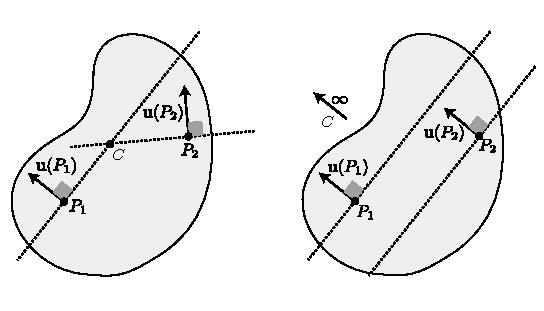
\includegraphics[scale=1.1]{Parti/P03-Meccanica_SR/C01-Cinematica_CR/Figure/chasles}
	\caption{Costruzioni grafica del centro di rotazione. Noti gli spostamenti di due punti $P_1$ e $P_2$ (sinistra) non paralleli, il centro di rotazione è univocamente determinato.
	Nel caso di traslazione pura (destra) il centro è improprio.}
	\label{fig:chasles}
\end{figure}


Se invece $\ub(P_1)\parallel\ub(P_2)$, si distinguono due casi: se ciò
accade per \emph{ogni} coppia di punti, allora $\vartheta=0$ e siamo nel caso di traslazione pura.
Tutte le rette così costruite
sono fra loro parallele, senza intersezione finita, coerentemente con un
centro improprio. Se invece $\vartheta\neq0$ e la coincidenza riguarda
solo $P_1,P_2$, vuol dire che $P_1$, $P_2$ e $C$ sono allineati (essendo
$\ub(P)=\bm\upvartheta\times\overrightarrow{CP}$), e le due rette non
bastano a determinare $C$: occorre un terzo punto non allineato con i
primi due.

%Questa costruzione è il caso a un solo corpo della \textit{cinematica
%	grafica}\index{cinematica grafica} dei sistemi rigidi piani, che
%ritroveremo, per sistemi di più corpi, in sez.~\ref{sec:CR_relativo}.







\subsection{Composizione di rotazioni infinitesime nel piano}\index{rotazione!composizione di rotazioni infinitesime|textbf}

Il campo di spostamento generato da più rotazioni infinitesime simultanee ha una
struttura sorprendentemente semplice.
Consideriamo $n$ rotazioni infinitesime nel piano, ciascuna di ampiezza $\vartheta_i$
e centro $C_i$, con $i = 1,\dots,n$. Poiché le rotazioni infinitesime commutano, lo
spostamento complessivo di un punto generico $P$ è la somma degli spostamenti
elementari:
\begin{equation}\label{eq:comp_rot_somma}
	\ub(P) = \sum_{i=1}^{n} \vartheta_i\,
	(\ab_z \times \overrightarrow{C_i P}).
\end{equation}
Scriviamo $\overrightarrow{C_i P} = \overrightarrow{OP} - \overrightarrow{OC_i}$
per un punto $O$ qualsiasi:
\begin{equation}
	\ub(P) =
	\Bigl(\sum_{i=1}^{n} \vartheta_i\Bigr)
	(\ab_z \times \overrightarrow{OP})
	- \sum_{i=1}^{n} \vartheta_i\,
	(\ab_z \times \overrightarrow{OC_i}).
\end{equation}
Posto
\begin{equation}\label{eq:comp_rot_theta}
	\vartheta = \sum_{i=1}^{n} \vartheta_i
\end{equation}
e, per $\vartheta \neq 0$,
\begin{equation}\label{eq:comp_rot_baricentro}
	\overrightarrow{OC}
	= \frac{1}{\vartheta}\sum_{i=1}^{n}
	\vartheta_i\,\overrightarrow{OC_i},
\end{equation}
lo spostamento complessivo diventa
\begin{equation}
	\ub(P) = \vartheta\,
	(\ab_z \times \overrightarrow{OP})
	- \vartheta\,
	(\ab_z \times \overrightarrow{OC})
	= \vartheta\,\ab_z \times
	(\overrightarrow{OP} - \overrightarrow{OC})
	= \vartheta\,\ab_z \times \overrightarrow{CP},
\end{equation}
ovvero
\begin{equation}\label{eq:comp_rot_risultato}
\ub(P)
		= \bm{\upvartheta} \times \overrightarrow{CP},
\end{equation}
cioè in componenti
\begin{equation}
u(P) = -\vartheta (y(P)- y(C)), \qquad
		v(P) = \vartheta (x(P)-x(C)).
\end{equation}
La composizione di $n$ rotazioni infinitesime è dunque una rotazione infinitesima di
ampiezza $\vartheta$ pari alla somma delle ampiezze (positive se antiorarie, negative
se orarie), il cui centro $C$ è il baricentro dei centri $C_i$ pesati con le
rispettive ampiezze $\vartheta_i$ (\FIGref{fig:composizione_rot}). La
\eqref{eq:comp_rot_baricentro} è indipendente dalla scelta del punto $O$, come si
verifica immediatamente sostituendo un diverso punto di riferimento.

\begin{figure}[!htbp]
	\centering
	\def\ax{0.5}\def\ay{0.30}
	\newcommand{\xyz}[3]{{#2 + (#1)*\ax},{#3 + (#1)*\ay}}
	\tikzset{midarrow/.style={postaction={decorate},decoration={markings, mark=at position 0.56 with {\arrow{Stealth}}}}}
	\resizebox{\textwidth}{!}{%
		\begin{tikzpicture}[baseline=(current bounding box.center),>=Stealth, line width=0.8pt, scale=1.1]
			\def\ax{0.5}\def\ay{-0.30}
			\begin{scope}[local bounding box=panA]
				\draw[gray!60] (\xyz{-1.5}{-0.9}{0}) -- (\xyz{-1.5}{4.7}{0})-- (\xyz{4.5}{4.7}{0}) -- (\xyz{4.5}{-0.9}{0}) -- cycle;
				\node[gray!75] at (\xyz{4.35}{4.5}{0}) {$\pi$};
				\coordinate (O) at (\xyz{0}{0}{0});
				\draw[->, thin] (O) -- (\xyz{0.9}{0}{0})  node[below right=-2pt] {$\ab_x$};
				\draw[->, thin] (O) -- (\xyz{0}{0.9}{0})  node[above=0pt]       {$\ab_y$};
				\draw[->, thin] (O) -- (\xyz{0}{0}{1.05}) node[left=-1pt]       {$\ab_z$};
				\newcommand{\axvec}[8]{%
					\coordinate (#1)  at (\xyz{#2}{#3}{0});
					\coordinate (#1t) at (\xyz{#2}{#3}{#4});
					\draw[->>, #8] (#1) -- (#1t) node[right=0pt, inner sep=1pt] {#6};
					\fill (#1) circle (1.4pt) node[#7, inner sep=1pt] {#5};
				}
				\axvec{C1}{2.6}{-0.02}{0.7}{$C_1$}{$\bm{\upvartheta}_1$}{below=2pt}{thick}
				\axvec{Ci}{0.9}{3.6}{0.7}{$C_i$}{$\bm{\upvartheta}_i$}{below right=-2pt}{thick}
				\axvec{Cn}{2.8}{3.9}{0.7}{$C_n$}{$\bm{\upvartheta}_n$}{below=2pt}{thick}
				\axvec{CC}{1.8}{2.3}{1.5}{}{$\bm{\upvartheta}=\textstyle\sum_i\bm{\upvartheta}_i$}{below=2pt}{line width=1.3pt}
				\fill (CC) circle (1.9pt) node[below=2pt, inner sep=1pt] {$C$};
				\draw[gray!75, thin, midarrow] (O) -- (Ci);
				\node[gray!75, font=\small, above] at ($(O)!0.86!(Ci)+(-0.75,0)$) {$\overrightarrow{OC_i}$};
				\draw[->, gray!30!black, thin] (O) -- (CC);
				\node[font=\small, below=1.5pt] at ($(O)!0.58!(CC)+(0.35,0)$) {$\overrightarrow{OC}$};
				\fill (O) circle (1.5pt) node[above left=-2pt] {$O$};
			\end{scope}
			\begin{scope}[xshift=8.6cm, yshift=-1.05cm, local bounding box=panB]
				\draw[->, thin] (-0.3,0) -- (5.4,0) node[right] {$x$};
				\draw[->, thin] (0,-0.3) -- (0,3.4) node[above] {$y$};
				\coordinate (C1) at (2.10,0.4);
				\coordinate (Ci) at (1.8,2.6);
				\coordinate (Cn) at (4.6,1.7);
				\coordinate (CC) at (2.4667,1.8667);
				\draw[->,gray!60, thin, midarrow] (CC)--(C1);
				\draw[->,gray!60, thin] (CC)--(Ci);
				\draw[->,gray!60, thin, midarrow] (CC)--(Cn);
				\newcommand{\rotc}[4]{%
					\draw[->, thick] ([shift={(-30:#2)}]#1)
					arc[start angle=-30, end angle=210, radius=#2];
					\node[inner sep=1pt] at ([shift={(#4:#2+0.20)}]#1) {#3};
				}
				\rotc{C1}{0.30}{$\vartheta_1$}{150}
				\rotc{Ci}{0.30}{$\vartheta_i$}{95}
				\rotc{Cn}{0.30}{$\vartheta_n$}{95}
				\rotc{CC}{0.42}{}{0}
				\node[inner sep=1pt] at ([shift={(0.6,0.60)}]CC) {$\vartheta=\textstyle\sum_i\vartheta_i$};
				\fill (C1) circle (1.5pt) node[below] {$C_1$};
				\fill (Ci) circle (1.5pt) node[left=10pt]       {$C_i$};
				\fill (Cn) circle (1.5pt) node[below]      {$C_n$};
				\fill (CC) circle (1.9pt) node[below=4pt]      {$C$};
				\draw[->, gray!30!black, thin] (0,0) -- (CC);
				\node[font=\small, above=1.5pt] at ($(0,0)!0.55!(CC)$) {$\overrightarrow{OC}$};
				\fill (0,0) circle (1.3pt) node[below left=-2pt] {$O$};
			\end{scope}
			\path let \p1=(panA.south), \p2=(panB.south) in	coordinate (ybase) at (0,{min(\y1,\y2)-12pt});
			\node[anchor=north] at (panA.south |- ybase) {(a)};
			\node[anchor=north] at (panB.south |- ybase) {(b)};
		\end{tikzpicture}
	}
	\caption{Composizione di $n$ rotazioni infinitesime nel piano.
		(a)~Vista tridimensionale: le rotazioni sono vettori assiali
		$\bm{\upvartheta}_i$ ortogonali al piano $\pi$, che si sommano nella
		risultante $\bm{\upvartheta}=\protect\sum_i\bm{\upvartheta}_i$ in $C$.
		(b)~Vista nel piano $(x,y)$: ampiezze $\vartheta_i$ come archi orientati
		(positivi se antiorari) e centro risultante $C$ nel baricentro dei $C_i$.
		Il centro $C$ è individuato da $\protect\overrightarrow{OC}=\protect\bigl(
		\protect\sum_i\vartheta_i\,\protect\overrightarrow{OC_i}\protect\bigr)/\vartheta$
		o, in forma equivalente, da $\protect\sum_i\vartheta_i\,
		\protect\overrightarrow{CC_i}=\zerovb$ (frecce grigie in~(b)).}
	\label{fig:composizione_rot}
\end{figure}

Se la somma delle ampiezze è nulla ($\vartheta = 0$), il baricentro
\eqref{eq:comp_rot_baricentro} non è definito: lo spostamento risultante è una
traslazione pura. Dalla \eqref{eq:comp_rot_somma} con $\sum\vartheta_i = 0$:
\begin{equation}
	\ub(P) = -\sum_{i=1}^{n} \vartheta_i\,
	(\ab_z \times \overrightarrow{OC_i}),
\end{equation}
indipendente da $P$: tutti i punti hanno lo stesso spostamento, coerentemente con
l'interpretazione del centro di rotazione all'infinito.

\begin{oss}
	La sovrapposizione~\eqref{eq:comp_rot_somma} richiede che ciascuna rotazione sia
	applicata alla configurazione iniziale del corpo, non alla configurazione variata
	dalle rotazioni precedenti. Questa procedura è lecita perché le rotazioni sono
	infinitesime: vista la linearità, le rotazioni infinitesime commutano e si sommano
	come vettori, dunque l'ordine di applicazione è irrilevante e la sovrapposizione
	degli effetti è esatta al primo ordine. Per rotazioni finite, al contrario, la
	composizione dipenderebbe dall'ordine e la semplice somma degli spostamenti non
	sarebbe corretta.
\end{oss}


\section{Centro di rotazione relativo e allineamento dei centri}\label{sec:CR_relativo}

Consideriamo un sistema di $n$ corpi rigidi $\mathcal{C}_1,\ldots,\mathcal{C}_n$ che
si muovono nel piano. Indichiamo con $i,j,k,\ldots\in\{1,\ldots,n\}$, a due a
due distinti, indici generici che identificano due o più corpi qualsiasi del
sistema: la costruzione che segue non dipende da quali, in particolare, siano stati
scelti.

Quando due corpi rigidi $\mathcal{C}_i$ e $\mathcal{C}_j$ si muovono nel piano,
ciascun punto dello spazio riceve in generale due spostamenti diversi: quello
che avrebbe come punto solidale al corpo $\mathcal{C}_i$ e quello che avrebbe
come punto solidale al corpo $\mathcal{C}_j$ (Oss.~\ref{spaziosolidale}). La
differenza fra i due è lo \textit{spostamento
	relativo}\index{spostamento!relativo} del corpo $\mathcal{C}_i$ rispetto al corpo
$\mathcal{C}_j$ in quel punto: è lo spostamento che un osservatore solidale
con il corpo $\mathcal{C}_j$ attribuisce al corpo $\mathcal{C}_i$.

Se i due corpi hanno rotazioni $\vartheta_i$ e $\vartheta_j$, la \textit{rotazione
	relativa}\index{rotazione!relativa} del corpo $\mathcal{C}_i$ rispetto al corpo
$\mathcal{C}_j$ è $\vartheta_i - \vartheta_j$. Questa semplice sottrazione è lecita
perché le rotazioni sono infinitesime e dunque si sommano (e si sottraggono) come
scalari. Per rotazioni finite, la composizione non sarebbe così immediata.

Il campo degli spostamenti relativi è esso stesso un campo rigido piano: essendo
differenza di due campi rigidi, è una funzione affine della posizione con la stessa
struttura della formula fondamentale. Possiede dunque un centro di rotazione (se
$\vartheta_i \neq \vartheta_j$) o è una traslazione pura (se
$\vartheta_i = \vartheta_j$).

\medskip

Siano $\vartheta_i$ e $\vartheta_j$ le ampiezze di rotazione dei due corpi, con
centri di rotazione $C_i$ e $C_j$. Lo spostamento di un punto generico $P$, solidale
al corpo $\mathcal{C}_i$ o al corpo $\mathcal{C}_j$, è dato dalla formula
fondamentale valutata rispetto al centro del corpo corrispondente:
\begin{equation}\label{eq:campi_assoluti_ij}
	\ub_i(P) = \vartheta_i\,\ab_z \times
	\overrightarrow{C_i P}, \qquad
	\ub_j(P) = \vartheta_j\,\ab_z \times
	\overrightarrow{C_j P}.
\end{equation}
Lo spostamento relativo del corpo $\mathcal{C}_i$ rispetto al corpo $\mathcal{C}_j$
nel punto $P$ è la differenza:
\begin{equation}\label{eq:spost_relativo}
	\ub_{ij}(P) = \ub_i(P) - \ub_j(P).
\end{equation}

Definiamo \textit{centro di rotazione relativo}\index{centro di rotazione!relativo|textbf}
$C_{ij}$  il punto in cui i due corpi hanno lo stesso spostamento assoluto:
\begin{equation}\label{eq:def_CR_relativo}
	\ub_i(C_{ij}) = \ub_j(C_{ij}),
\end{equation}
ovvero il punto in cui lo spostamento relativo si annulla: $\ub_{ij}(C_{ij}) =
\zerovb$. Due punti materiali, uno solidale al corpo $\mathcal{C}_i$ e l'altro al
corpo $\mathcal{C}_j$, che nella configurazione iniziale coincidono in $C_{ij}$,
restano sovrapposti dopo lo spostamento.

\subsection{Primo teorema di Aronhold-Kennedy: allineamento dei centri assoluti}
Valutiamo le due espressioni~\eqref{eq:campi_assoluti_ij} nel punto $C_{ij}$:
\begin{equation}
	\ub_i(C_{ij}) = \vartheta_i\,\ab_z\times\overrightarrow{C_iC_{ij}}, \qquad
	\ub_j(C_{ij}) = \vartheta_j\,\ab_z\times\overrightarrow{C_jC_{ij}}.
\end{equation}
Per la definizione di centro relativo~\eqref{eq:def_CR_relativo} i due membri di
destra coincidono:
\begin{equation}
	\vartheta_i\,\ab_z\times\overrightarrow{C_iC_{ij}}
	= \vartheta_j\,\ab_z\times\overrightarrow{C_jC_{ij}}.
\end{equation}
L'applicazione $\wb\mapsto\ab_z\times\wb$ è lineare e iniettiva sul piano (è una
rotazione di $\pi/2$, che conserva il modulo e dunque annulla solo il vettore
nullo); possiamo perciò eliminarla da entrambi i membri:
\begin{equation}\label{eq:CR_relativo_scalare}
	\vartheta_i\,\overrightarrow{C_iC_{ij}}
	= \vartheta_j\,\overrightarrow{C_jC_{ij}}.
\end{equation}
Se $\vartheta_i=\vartheta_j$, questa condizione impone $C_i=C_j$: per centri
distinti non esiste dunque, in questo caso, un punto a distanza finita in cui i due
spostamenti coincidano --- coerentemente con il caso limite della traslazione
relativa pura. Se invece $\vartheta_i\neq\vartheta_j$, scrivendo
$\overrightarrow{C_jC_{ij}} = \overrightarrow{C_iC_{ij}} - \overrightarrow{C_iC_j}$
nella~\eqref{eq:CR_relativo_scalare} e risolvendo per $\overrightarrow{C_iC_{ij}}$
si ottiene
\begin{equation}\label{eq:CR_relativo_pos}
	\overrightarrow{C_i C_{ij}}
	= -\frac{\vartheta_j}{\vartheta_i - \vartheta_j}\,
	\overrightarrow{C_i C_j}.
\end{equation}
Poiché $\overrightarrow{C_iC_{ij}}$ è proporzionale a $\overrightarrow{C_iC_j}$, i
tre punti $C_i$, $C_j$ e $C_{ij}$ sono \textit{allineati}
(\FIGref{fig:allineamento_CR}). Questo risultato va sotto il nome di \textit{primo teorema di Aronhold-Kennedy}. \index{teorema!di Aronhold-Kennedy (primo)|textbf}

\begin{oss}
	La posizione di $C_{ij}$ si ritrova anche specializzando a $n=2$ la formula
	generale di composizione~\eqref{eq:comp_rot_baricentro}: lo spostamento
	relativo~\eqref{eq:spost_relativo} è la composizione di una rotazione
	$\vartheta_i$ attorno a $C_i$ e di una rotazione $-\vartheta_j$ attorno a
	$C_j$ (il segno meno riflette quello nella~\eqref{eq:spost_relativo}).
	Applicando la~\eqref{eq:comp_rot_baricentro} con pesi $\vartheta_i$ e
	$-\vartheta_j$ si ritrova immediatamente la~\eqref{eq:CR_relativo_pos}.
\end{oss}

\begin{figure}[htbp]
	\centering
	\subfloat[]{%
		\begin{tikzpicture}[>=Stealth, line width=0.8pt, scale=1.0]
			\draw[dashed, gray!50] (-0.8,0) -- (4.5,0);
			\fill (0,0)  circle (2pt) node[below=5pt] {$C_i$};
			\fill (3,0)  circle (2pt) node[below=5pt] {$C_j$};
			\fill (2,0)  circle (2pt) node[below=5pt] {$C_{ij}$};
			\draw[<->, thin] (0,-1.0) -- (2,-1.0) node[midway, below] {\small$\tfrac{2}{3}|C_iC_j|$};
			\draw[<->, thin] (2,-1.0) -- (3,-1.0) node[midway, below] {\small$\tfrac{1}{3}|C_iC_j|$};
			\draw[->, thick] (-0.5,0.1) arc[start angle=160, end angle=20, radius=0.55];
			\node[above] at (0,0.65) {\small$\vartheta_i$};
			\draw[->, thick] (3.5,0.1) arc[start angle=20, end angle=160, radius=0.55];
			\node[above] at (3,0.65) {\small$\vartheta_j{=}{-}2\vartheta_i$};
	\end{tikzpicture}}%
	\hspace{0.06\textwidth}%
	\subfloat[]{%
		\begin{tikzpicture}[>=Stealth, line width=0.8pt, scale=1.0]
			\draw[dashed, gray!50] (-0.8,0) -- (5.5,0);
			\fill (0,0)  circle (2pt) node[below=5pt] {$C_i$};
			\fill (2,0)  circle (2pt) node[below=5pt] {$C_j$};
			\fill (4,0)  circle (2pt) node[below=5pt] {$C_{ij}$};
			\draw[thick] (0,0) -- (2,0);
			\draw[<->, thin] (0,-1.0) -- (2,-1.0) node[midway, below] {\small$|C_iC_j|$};
			\draw[<->, thin] (0,-1.6) -- (4,-1.6) node[midway, below] {\small$2|C_iC_j|$};
			\draw[->, thick] (-0.5,0.1) arc[start angle=160, end angle=20, radius=0.55];
			\node[above] at (0,0.65) {\small$\vartheta_i$};
			\draw[->, thick] (1.5,0.1) arc[start angle=160, end angle=20, radius=0.55];
			\node[above] at (2,0.65) {\small$\vartheta_j{=}2\vartheta_i$};
	\end{tikzpicture}}
	\caption{Allineamento dei centri di rotazione $C_i$, $C_j$ e $C_{ij}$
		con $|\vartheta_j| = 2|\vartheta_i|$.
		\textbf{\textit{(a)}}~Rotazioni discordi ($\vartheta_i > 0$,
		$\vartheta_j = -2\vartheta_i$): $C_{ij}$ cade all'interno del segmento
		$C_iC_j$, a distanza $\tfrac{2}{3}|C_iC_j|$ da $C_i$.
		\textbf{\textit{(b)}}~Rotazioni concordi ($\vartheta_i > 0$,
		$\vartheta_j = 2\vartheta_i$): $C_{ij}$ cade all'esterno, oltre $C_j$,
		a distanza $2|C_iC_j|$ da $C_i$.}
	\label{fig:allineamento_CR}
\end{figure}

\begin{oss}[\textbf{Posizione del centro relativo}]
	Il segno del coefficiente $-\vartheta_j/(\vartheta_i-\vartheta_j)$ nella
	\eqref{eq:CR_relativo_pos} determina la posizione di $C_{ij}$ sulla retta
	$C_iC_j$:
	\begin{enumerate}[label=(\alph*)]
		\item se $\vartheta_i$ e $\vartheta_j$ sono concordi, il coefficiente è
		esterno all'intervallo $(0,1)$ e $C_{ij}$ cade \textit{all'esterno} del
		segmento $C_i C_j$, dalla parte del centro con rotazione di valore assoluto
		maggiore;
		\item  se $\vartheta_i$ e $\vartheta_j$ sono discordi, il coefficiente è
		compreso fra $0$ e $1$ e $C_{ij}$ cade \textit{all'interno} del segmento
		$C_i C_j$;
		\item  se $\vartheta_i = \vartheta_j$, $C_{ij}$ è all'infinito nella direzione
		di $\overrightarrow{C_i C_j}$: lo spostamento relativo è una traslazione
		pura, perpendicolare alla congiungente dei centri, di modulo
		$|\vartheta_i|\,|\overrightarrow{C_i C_j}|$.
	\end{enumerate}
\end{oss}

\begin{oss}
	La proprietà di allineamento $C_i$--$C_{ij}$--$C_j$ è il fondamento della
	\textit{cinematica grafica}\index{cinematica grafica|textbf} dei sistemi di corpi
	rigidi piani: nota la posizione di due centri, il terzo si trova come
	intersezione di rette. Inoltre, dalla~\eqref{eq:CR_relativo_pos}, noti i tre
	centri e la rotazione $\vartheta_i$ di uno dei due corpi, la rotazione
	dell'altro è univocamente determinata:
	\begin{equation}\label{eq:rot_da_centri}
		\vartheta_j = \vartheta_i\,
		\frac{|\overrightarrow{C_j C_{ij}}|}
		{|\overrightarrow{C_i C_{ij}}|},
	\end{equation}
	con segno positivo se $C_{ij}$ è esterno al segmento $C_i C_j$ (rotazioni
	concordi), negativo se interno (rotazioni discordi). L'allineamento dei centri
	fornisce dunque sia la geometria che l'ampiezza degli spostamenti rigidi. 
	
	\begin{figure}[htbp]
		\centering
		\subfloat[][\emph{$C_{ij}$ interno: rotazioni discordi}]{%
			\begin{tikzpicture}[>=Stealth, line width=0.8pt, scale=0.95]
				\def\ang{22}
				\def\tg{0.4040}
				\coordinate (Ci)      at (0,0);
				\coordinate (Cij)     at (2,0);
				\coordinate (Cj)      at (3,0);
				\coordinate (Cij_up)  at (2, {2*\tg});
				\draw[dashed, gray!60] (-0.5,0) -- (4.2,0);
				\draw[gray!50] (Ci) -- ({3.8*cos(\ang)}, {3.8*sin(\ang)});
				\draw[->, thick] (0.9,0) arc[start angle=0, end angle=\ang, radius=0.9];
				\node[right=1pt] at (0.85,0.20) {\small$\vartheta_i$};
				\draw[<-, thick] ({3+0.7*cos(141)},{0.7*sin(141)}) arc[start angle=141, end angle=180, radius=0.7];
				\node at ({4-1.42},{0.15}) {\small$\vartheta_j$};
				\draw[->, dashed, thick] (Cij) -- (Cij_up);
				\draw[thick, gray!60] (Cj) -- (Cij_up);
				\fill (Ci)     circle (2pt) node[below=5pt] {$C_i$};
				\fill (Cij)    circle (2pt) node[below=5pt] {$C_{ij}$};
				\fill (Cj)     circle (2pt) node[below=5pt] {$C_j$};
				\fill (Cij_up) circle (2pt);
		\end{tikzpicture}}%
		\hspace{0.03\textwidth}%
		\subfloat[][\emph{$C_{ij}$ esterno: rotazioni concordi}]{%
			\begin{tikzpicture}[>=Stealth, line width=0.8pt, scale=0.95]
				\def\ang{22}
				\def\tg{0.4040}
				\coordinate (Ci)      at (0,0);
				\coordinate (Cj)      at (2,0);
				\coordinate (Cij)     at (4,0);
				\coordinate (Cij_up)  at (4, {4*\tg});
				\draw[dashed, gray!60] (-0.5,0) -- (5.2,0);
				\draw[gray!50] (Ci) -- ({4.8*cos(\ang)}, {4.8*sin(\ang)});
				\draw[->, thick] (0.9,0) arc[start angle=0, end angle=\ang, radius=0.9];
				\node[right=1pt] at (0.85,0.20) {\small$\vartheta_i$};
				\draw[->, thick] ({2+0.7},0) arc[start angle=0, end angle=39, radius=0.7];
				\node at ({2+0.95},0.20) {\small$\vartheta_j$};
				\draw[->, dashed, thick] (Cij) -- (Cij_up);
				\draw[thick, gray!60] (Cj) -- (Cij_up);
				\fill (Ci)     circle (2pt) node[below=5pt] {$C_i$};
				\fill (Cj)     circle (2pt) node[below=5pt] {$C_j$};
				\fill (Cij)    circle (2pt) node[below=5pt] {$C_{ij}$};
				\fill (Cij_up) circle (2pt);
		\end{tikzpicture}}
		\caption{Cinematica grafica: determinazione di $\vartheta_j$ dalla posizione
			dei centri e da $\vartheta_i$. La retta $C_iC_{ij}C_j$ ruota di $\vartheta_i$
			attorno a $C_i$; lo spostamento verticale di $C_{ij}$ è proporzionale
			alla sua distanza da $C_i$. La retta grigia da $C_j$ alla posizione ruotata
			di $C_{ij}$ evidenzia per similitudine il rapporto
			$|\vartheta_j|/|\vartheta_i| = |C_jC_{ij}|/|C_iC_{ij}|$.}
		\label{fig:cinematica_grafica}
	\end{figure}
\end{oss}


\subsection{Secondo teorema di Aronhold-Kennedy: allineamento dei centri relativi}
\label{sec:allineamento_relativi}
\index{allineamento dei centri di rotazione|textbf}\index{teorema!di Aronhold-Kennedy (secondo)|textbf}

Consideriamo tre corpi rigidi $\mathcal{C}_i$, $\mathcal{C}_j$, $\mathcal{C}_k$ nel
piano, con rotazioni $\vartheta_i$, $\vartheta_j$, $\vartheta_k$ e centri di
rotazione assoluti\index{centro di rotazione!assoluto} $C_i$, $C_j$, $C_k$. I centri
di rotazione relativi $C_{ij}$, $C_{ik}$, $C_{jk}$ sono definiti come nella
Sezione~\ref{sec:CR_relativo}: $C_{ij}$ è il punto di uguale spostamento per i corpi
$\mathcal{C}_i$ e $\mathcal{C}_j$, e così via.

Il \textit{secondo teorema di Aronhold-Kennedy} stabilisce che i tre centri di rotazione relativi $C_{ij}$, $C_{ik}$ e $C_{jk}$ sono allineati.

\medskip 

Supponiamo $\vartheta_i,\vartheta_j,\vartheta_k$ a due a due distinti (altrimenti
una delle tre coppie di corpi è in traslazione relativa pura, e il centro relativo
corrispondente è improprio). Scrivendo la~\eqref{eq:CR_relativo_pos} in termini di
vettori posizione rispetto a un punto $O$ fissato ad arbitrio, per ciascuna coppia
di corpi si ottiene
\begin{equation}\label{eq:tre_centri_pos}
\begin{aligned}
	&	\overrightarrow{OC_{ij}} = \frac{\vartheta_i\overrightarrow{OC_i}-\vartheta_j\overrightarrow{OC_j}}{\vartheta_i-\vartheta_j}, \qquad
	\overrightarrow{OC_{jk}} = \frac{\vartheta_j\overrightarrow{OC_j}-\vartheta_k\overrightarrow{OC_k}}{\vartheta_j-\vartheta_k},\\
&	\overrightarrow{OC_{ik}} = \frac{\vartheta_i\overrightarrow{OC_i}-\vartheta_k\overrightarrow{OC_k}}{\vartheta_i-\vartheta_k}.
\end{aligned}
\end{equation}
Poniamo
\begin{equation}
	a:=\vartheta_i-\vartheta_j, \qquad b:=\vartheta_j-\vartheta_k, \qquad c:=\vartheta_k-\vartheta_i,
\end{equation}
sicché $a+b+c=0$ identicamente. Moltiplicando ciascuna delle~\eqref{eq:tre_centri_pos}
per il proprio denominatore,
\begin{equation}
\begin{aligned}
	&	a\,\overrightarrow{OC_{ij}} = \vartheta_i\overrightarrow{OC_i}-\vartheta_j\overrightarrow{OC_j}, \qquad
	b\,\overrightarrow{OC_{jk}} = \vartheta_j\overrightarrow{OC_j}-\vartheta_k\overrightarrow{OC_k}, \\
&	c\,\overrightarrow{OC_{ik}} = \vartheta_k\overrightarrow{OC_k}-\vartheta_i\overrightarrow{OC_i},
\end{aligned}
\end{equation}
e sommando membro a membro, i termini a destra si elidono a due a due:
\begin{equation}\label{eq:allineamento_somma_nulla}
	a\,\overrightarrow{OC_{ij}} + b\,\overrightarrow{OC_{jk}} + c\,\overrightarrow{OC_{ik}} = \zerovb,
	\qquad a+b+c=0.
\end{equation}
Sostituendo $c=-a-b$ nella~\eqref{eq:allineamento_somma_nulla} e raccogliendo,
\begin{equation}
	a\,(\overrightarrow{OC_{ij}}-\overrightarrow{OC_{ik}})
	+ b\,(\overrightarrow{OC_{jk}}-\overrightarrow{OC_{ik}}) = \zerovb,
	\qquad\text{cioè}\qquad
	a\,\overrightarrow{C_{ik}C_{ij}} = -b\,\overrightarrow{C_{ik}C_{jk}}.
\end{equation}
Poiché $a=\vartheta_i-\vartheta_j\neq 0$ e $b=\vartheta_j-\vartheta_k\neq\mathbf{0}$ per ipotesi, 
$\overrightarrow{C_{ik}C_{ij}}$ è  multiplo di $\overrightarrow{C_{ik}C_{jk}}$,
cioè
\begin{equation}
	C_{ij},\; C_{ik},\; C_{jk} \quad \text{sono allineati.}
\end{equation}

\begin{figure}[htbp]
	\centering
	\begin{tikzpicture}[>=Stealth, line width=0.8pt, scale=1.1]
		\coordinate (Ci)  at (1.000, 0.500);
		\coordinate (Cj)  at (4.500, 0.000);
		\coordinate (Ck)  at (1.500, 3.500);
		\coordinate (Cij) at (5.550, -0.150);
		\coordinate (Cik) at (1.350,  2.600);
		\coordinate (Cjk) at (3.450,  1.225);
		\coordinate (ext1) at (0.090,  3.425);
		\coordinate (ext2) at (4.710,  0.400);
		\draw[gray!40, dashed] (-0.050, 0.650) -- (Ci) -- (Cj) -- (Cij) -- (6.100, -0.300);
		\draw[gray!40, dashed] (0.850, -0.500) -- (Ci) -- (Ck) -- (1.650, 4.400);
		\draw[gray!40, dashed] (5.400, -1.050) -- (Cj) -- (Ck) -- (0.600, 4.550);
		\draw[thick, gray!60] (ext1) -- (Cik) -- (Cjk) -- (Cij) -- (6.600, -0.838);
		\fill (Ci) circle (2.5pt);
		\fill (Cj) circle (2.5pt);
		\fill (Ck) circle (2.5pt);
		\node[below left=3pt] at (Ci) {$C_i$};
		\node[below=4pt]       at (Cj) {$C_j$};
		\node[right=4pt]       at (Ck) {$C_k$};
		\fill[white] (Cij) circle (3pt);
		\draw[thick]  (Cij) circle (3pt);
		\fill[white] (Cik) circle (3pt);
		\draw[thick]  (Cik) circle (3pt);
		\fill[white] (Cjk) circle (3pt);
		\draw[thick]  (Cjk) circle (3pt);
		\node[above=4pt] at (Cij) {$C_{ij}$};
		\node[left=4pt]        at (Cik) {$C_{ik}$};
		\node[above right=2pt] at (Cjk) {$C_{jk}$};
	\end{tikzpicture}
	\caption{Teorema di allineamento dei centri di rotazione relativi.
		I tre corpi $\mathcal{C}_i$, $\mathcal{C}_j$, $\mathcal{C}_k$ hanno centri
		assoluti $C_i$, $C_j$, $C_k$ (cerchi pieni). I centri di rotazione relativi
		$C_{ij}$, $C_{ik}$, $C_{jk}$ --- ciascuno punto di uguale spostamento per la
		coppia di corpi corrispondente --- sono allineati (cerchi vuoti, retta
		grigia). Il centro $C_{ij}$ cade all'esterno del segmento $C_iC_j$,
		coerentemente con il teorema di Menelao.}
	\label{fig:allineamento_relativi}
\end{figure}

\begin{oss}
	Il risultato è del tutto generale: vale per qualsiasi terna di corpi rigidi nel
	piano, indipendentemente dal fatto che siano connessi fra loro o meno. Quando
	uno dei tre corpi è il suolo (corpo $0$, con $\vartheta_0 = 0$), i centri
	relativi $C_{i0}$ e $C_{j0}$ coincidono con i centri assoluti $C_i$ e $C_j$, e il
	teorema si riduce all'allineamento $C_i$--$C_{ij}$--$C_j$ già dimostrato.
\end{oss}

\begin{oss}
	Il teorema a tre corpi ammette anche una dimostrazione che riusa il teorema a
	due corpi, applicandolo non ai corpi originali ma a una coppia di campi
	costruiti apposta. I campi $\ub_{ik}:=\ub_i-\ub_k$ e $\ub_{jk}:=\ub_j-\ub_k$
	sono rigidi (per lo stesso argomento visto per $\ub_{ij}$), di centri $C_{ik}$
	e $C_{jk}$, e si interpretano come gli spostamenti di $\mathcal{C}_i$ e
	$\mathcal{C}_j$ visti da un osservatore solidale con $\mathcal{C}_k$. La loro
	differenza è $\ub_{ik}-\ub_{jk}=\ub_i-\ub_j=\ub_{ij}$: applicando il teorema a
	due corpi alla coppia $(\ub_{ik},\ub_{jk})$ si ritrova che il suo zero, cioè
	$C_{ij}$, è allineato con $C_{ik}$ e $C_{jk}$.
\end{oss}


\begin{oss}
	Come nel caso di due corpi, l'allineamento dei centri relativi fornisce non
	solo la geometria ma anche le ampiezze. Noti i tre centri $C_{ij}$, $C_{ik}$,
	$C_{jk}$ e la rotazione $\vartheta_i$ di uno dei tre corpi, le rotazioni degli
	altri due sono univocamente determinate. Dalla~\eqref{eq:rot_da_centri}
	applicata alle coppie $(i,k)$ e $(i,j)$:
	\begin{equation}
		\vartheta_k = \vartheta_i\,
		\frac{|\overrightarrow{C_k C_{ik}}|}
		{|\overrightarrow{C_i C_{ik}}|}, \qquad
		\vartheta_j = \vartheta_i\,
		\frac{|\overrightarrow{C_j C_{ij}}|}
		{|\overrightarrow{C_i C_{ij}}|},
	\end{equation}
	con segni determinati dalla posizione interna o esterna dei centri relativi.
	L'allineamento dei centri è dunque uno strumento completo per l'analisi
	cinematica: le posizioni dei centri determinano la geometria degli spostamenti,
	i rapporti delle distanze ne determinano le ampiezze.
\end{oss}


	
	
\todo[inline]{Eliminerei gli esercizi}

%-------------------------------------------------------------------------------
\section{Esercizi proposti}
%-------------------------------------------------------------------------------

\begin{esercizio}[Spostamento rigido nello spazio]
	\label{ex:C01_spostamento_3D}
	
	Un corpo rigido subisce uno spostamento infinitesimo con $\ub(O) = (1\;\,0\;\,2)^\top$ e $\bm{\upvartheta} = (0\;\,0\;\,0.1)^\top$ (rotazione attorno a $\ab_z$). Posto $O$ nell'origine, calcolare lo spostamento del punto $P$ di coordinate $\bm{x}(P) = (3\;\,4\;\,0)^\top$:
	(a) con la formula vettoriale~\eqref{eq:FFCI};
	(b) con la forma matriciale~\eqref{eq:FFCI_estesa}.
	
	\risultato (a) $\bm{\upvartheta} \times \overrightarrow{OP} = (-0.4\;\,0.3\;\,0)^\top$, da cui $\ub(P) = (0.6\;\,0.3\;\,2)^\top$. (b) $\bm{\varTheta}\,\bm{x}(P) = (-0.4\;\,0.3\;\,0)^\top$, da cui $\bm{u}(P) = (0.6\;\,0.3\;\,2)^\top$. I due risultati coincidono.
	
\end{esercizio}

\begin{esercizio}[Verifica della condizione di ortogonalità]
	\label{ex:C01_ortogonalita}
	
	Per i dati dell'\ESEref{ex:C01_spostamento_3D}, scegliere un secondo punto $Q$ di coordinate $\bm{x}(Q) = (1\;\,5\;\,0)^\top$. Calcolare $\ub(Q)$ e verificare la condizione di ortogonalità~\eqref{eq:ortogonalita_CR}: $\overrightarrow{PQ} \cdot [\ub(Q) - \ub(P)] = 0$.
	
	\risultato $\bm{\upvartheta} \times \overrightarrow{OQ} = (-0.5\;\,0.1\;\,0)^\top$, da cui $\ub(Q) = (0.5\;\,0.1\;\,2)^\top$. $\overrightarrow{PQ} = (-2\;\,1\;\,0)^\top$, $\ub(Q) - \ub(P) = (-0.1\;\,-0.2\;\,0)^\top$, infine $\overrightarrow{PQ} \cdot [\ub(Q) - \ub(P)] = 0.2 - 0.2 = 0$.
	
\end{esercizio}

\begin{esercizio}[Invarianti del campo di spostamento]
	\label{ex:C01_invarianti}
	
	Per i dati dell'\ESEref{ex:C01_spostamento_3D}:
	(a) calcolare il primo invariante $\bm{\upvartheta}$ (già noto);
	(b) calcolare il secondo invariante $\bm{\upvartheta} \cdot \ub(O)$;
	(c) verificare che $\bm{\upvartheta} \cdot \ub(P) = \bm{\upvartheta} \cdot \ub(O)$;
	(d) classificare il moto rigido.
	
	\risultato (a) $\bm{\upvartheta} = (0\;\,0\;\,0.1)^\top$. (b) $\bm{\upvartheta} \cdot \ub(O) = 0.1 \cdot 2 = 0.2$. (c) $\bm{\upvartheta} \cdot \ub(P) = 0.1 \cdot 2 = 0.2$, coincide con il secondo invariante (b). (d) $\bm{\upvartheta} \neq \zerovb$ e $\bm{\upvartheta} \cdot \ub(O) \neq 0$: il moto è una \textit{rototraslazione}, con asse di rotazione parallelo a $\ab_z$ e componente di traslazione lungo $\ab_z$.
	
\end{esercizio}

\begin{esercizio}[Centro di rotazione nel piano]
	\label{ex:C01_CR_piano}
	
	Nel piano $(x,y)$, un corpo rigido ha spostamento del polo $\ub(O) = (0.3\;\,-0.6)^\top$ e rotazione $\vartheta = 0.1$\,rad.
	(a) Determinare le coordinate del centro di rotazione $C$ con la~\eqref{eq:CR_coord}.
	(b) Calcolare lo spostamento del punto $P = (5,\,2)$ sia con la~\eqref{eq:FFCI_piano} sia come $\bm{\upvartheta} \times \overrightarrow{CP}$ e verificare che i risultati coincidono.
	
	\risultato (a) $x(C) = -v(O)/\vartheta = 6$, $y(C) = u(O)/\vartheta = 3$, dunque $C = (6,\,3)$. (b) Con la~\eqref{eq:FFCI_piano}: $u(P) = 0.3 - 0.1 \cdot 2 = 0.1$, $v(P) = -0.6 + 0.1 \cdot 5 = -0.1$, da cui $\ub(P) = (0.1\;\,-0.1)^\top$. Con $\bm{\upvartheta} \times \overrightarrow{CP}$: $\overrightarrow{CP} = (-1\;\,-1\;\,0)^\top$, da cui $\bm{\upvartheta} \times \overrightarrow{CP} = (0.1\;\,-0.1\;\,0)^\top$. I due risultati coincidono.
	
\end{esercizio}

\begin{esercizio}[Traslazione pura]
	\label{ex:C01_traslazione}
	
	Un corpo rigido nel piano ha $\ub(O) = (2\;\,-1)^\top$ e $\vartheta = 0$.
	(a) Calcolare lo spostamento di tre punti a scelta.
	(b) Verificare che tutti hanno lo stesso spostamento.
	(c) Commentare la posizione del centro di rotazione.
	
	\risultato (a) Per qualsiasi $P$: $\ub(P) = \ub(O) + \bm{\upvartheta} \times \overrightarrow{OP} = \ub(O) + \zerovb = \ub(O)$. Per $P_1 = (0,\,0)$, $P_2 = (3,\,4)$, $P_3 = (-1,\,5)$ si ottiene $\ub(P_1) = \ub(P_2) = \ub(P_3) = (2\;\,-1)^\top$. (b) Tutti i punti hanno lo stesso spostamento. (c) La~\eqref{eq:CR_coord} è singolare per $\vartheta = 0$: il centro di rotazione è all'\textit{infinito}, in direzione perpendicolare allo spostamento. La traslazione pura è il limite della rotazione con centro di rotazione che si allontana indefinitamente.
	
\end{esercizio}

\begin{esercizio}[Dal campo di spostamento ai parametri]
	\label{ex:C01_inversione}
	
	Sono noti gli spostamenti di due punti di un corpo rigido piano: $\ub(A) = (0.1\;\,0.2)^\top$ con $A = (0,\,0)$ e $\ub(B) = (0.1\;\,0.3)^\top$ con $B = (1,\,0)$.
	(a) Dalla differenza $\ub(B) - \ub(A) = \bm{\upvartheta} \times \overrightarrow{AB}$, determinare la rotazione $\vartheta$.
	(b) Determinare le coordinate del centro di rotazione.
	(c) Verificare che $\ub(A) = \bm{\upvartheta} \times \overrightarrow{CA}$ e $\ub(B) = \bm{\upvartheta} \times \overrightarrow{CB}$.
	
	\risultato (a) $\overrightarrow{AB} = (1\;\,0)^\top$, $\ub(B) - \ub(A) = (0\;\,0.1)^\top$. La componente $y$ del prodotto vettoriale dà $\vartheta \cdot 1 = 0.1$, da cui $\vartheta = 0.1$\,rad. (b) Applicando la procedura della~\eqref{eq:CR_coord} ai dati di $A$: $y_C = y_A + u_A/\vartheta = 0 + 0.1/0.1 = 1$, $x_C = x_A - v_A/\vartheta = 0 - 0.2/0.1 = -2$, dunque $C = (-2,\,1)$. (c) $\overrightarrow{CA} = (2\;\,-1\;\,0)^\top$, $\bm{\upvartheta} \times \overrightarrow{CA} = (0.1\;\,0.2\;\,0)^\top = \ub(A)$. $\overrightarrow{CB} = (3\;\,-1\;\,0)^\top$, $\bm{\upvartheta} \times \overrightarrow{CB} = (0.1\;\,0.3\;\,0)^\top = \ub(B)$.
	
\end{esercizio}
	
	
	
